\documentclass[twoside]{book}

% Packages required by doxygen
\usepackage{fixltx2e}
\usepackage{calc}
\usepackage{doxygen}
\usepackage[export]{adjustbox} % also loads graphicx
\usepackage{graphicx}
\usepackage[utf8]{inputenc}
\usepackage{makeidx}
\usepackage{multicol}
\usepackage{multirow}
\PassOptionsToPackage{warn}{textcomp}
\usepackage{textcomp}
\usepackage[nointegrals]{wasysym}
\usepackage[table]{xcolor}

% Font selection
\usepackage[T1]{fontenc}
\usepackage[scaled=.90]{helvet}
\usepackage{courier}
\usepackage{amssymb}
\usepackage{sectsty}
\renewcommand{\familydefault}{\sfdefault}
\allsectionsfont{%
  \fontseries{bc}\selectfont%
  \color{darkgray}%
}
\renewcommand{\DoxyLabelFont}{%
  \fontseries{bc}\selectfont%
  \color{darkgray}%
}
\newcommand{\+}{\discretionary{\mbox{\scriptsize$\hookleftarrow$}}{}{}}

% Page & text layout
\usepackage{geometry}
\geometry{%
  a4paper,%
  top=2.5cm,%
  bottom=2.5cm,%
  left=2.5cm,%
  right=2.5cm%
}
\tolerance=750
\hfuzz=15pt
\hbadness=750
\setlength{\emergencystretch}{15pt}
\setlength{\parindent}{0cm}
\setlength{\parskip}{3ex plus 2ex minus 2ex}
\makeatletter
\renewcommand{\paragraph}{%
  \@startsection{paragraph}{4}{0ex}{-1.0ex}{1.0ex}{%
    \normalfont\normalsize\bfseries\SS@parafont%
  }%
}
\renewcommand{\subparagraph}{%
  \@startsection{subparagraph}{5}{0ex}{-1.0ex}{1.0ex}{%
    \normalfont\normalsize\bfseries\SS@subparafont%
  }%
}
\makeatother

% Headers & footers
\usepackage{fancyhdr}
\pagestyle{fancyplain}
\fancyhead[LE]{\fancyplain{}{\bfseries\thepage}}
\fancyhead[CE]{\fancyplain{}{}}
\fancyhead[RE]{\fancyplain{}{\bfseries\leftmark}}
\fancyhead[LO]{\fancyplain{}{\bfseries\rightmark}}
\fancyhead[CO]{\fancyplain{}{}}
\fancyhead[RO]{\fancyplain{}{\bfseries\thepage}}
\fancyfoot[LE]{\fancyplain{}{}}
\fancyfoot[CE]{\fancyplain{}{}}
\fancyfoot[RE]{\fancyplain{}{\bfseries\scriptsize Generated by Doxygen }}
\fancyfoot[LO]{\fancyplain{}{\bfseries\scriptsize Generated by Doxygen }}
\fancyfoot[CO]{\fancyplain{}{}}
\fancyfoot[RO]{\fancyplain{}{}}
\renewcommand{\footrulewidth}{0.4pt}
\renewcommand{\chaptermark}[1]{%
  \markboth{#1}{}%
}
\renewcommand{\sectionmark}[1]{%
  \markright{\thesection\ #1}%
}

% Indices & bibliography
\usepackage{natbib}
\usepackage[titles]{tocloft}
\setcounter{tocdepth}{3}
\setcounter{secnumdepth}{5}
\makeindex

% Hyperlinks (required, but should be loaded last)
\usepackage{ifpdf}
\ifpdf
  \usepackage[pdftex,pagebackref=true]{hyperref}
\else
  \usepackage[ps2pdf,pagebackref=true]{hyperref}
\fi
\hypersetup{%
  colorlinks=true,%
  linkcolor=blue,%
  citecolor=blue,%
  unicode%
}

% Custom commands
\newcommand{\clearemptydoublepage}{%
  \newpage{\pagestyle{empty}\cleardoublepage}%
}

\usepackage{caption}
\captionsetup{labelsep=space,justification=centering,font={bf},singlelinecheck=off,skip=4pt,position=top}

%===== C O N T E N T S =====

\begin{document}

% Titlepage & ToC
\hypersetup{pageanchor=false,
             bookmarksnumbered=true,
             pdfencoding=unicode
            }
\pagenumbering{alph}
\begin{titlepage}
\vspace*{7cm}
\begin{center}%
{\Large A\+C\+ME }\\
\vspace*{1cm}
{\large Generated by Doxygen 1.8.13}\\
\end{center}
\end{titlepage}
\clearemptydoublepage
\pagenumbering{roman}
\tableofcontents
\clearemptydoublepage
\pagenumbering{arabic}
\hypersetup{pageanchor=true}

%--- Begin generated contents ---
\chapter{Namespace Index}
\section{Namespace List}
Here is a list of all documented namespaces with brief descriptions\+:\begin{DoxyCompactList}
\item\contentsline{section}{\hyperlink{namespaceacme}{acme} }{\pageref{namespaceacme}}{}
\end{DoxyCompactList}

\chapter{Hierarchical Index}
\section{Class Hierarchy}
This inheritance list is sorted roughly, but not completely, alphabetically\+:\begin{DoxyCompactList}
\item \contentsline{section}{acme\+:\+:point$<$ T, D $>$}{\pageref{classacme_1_1point}}{}
\begin{DoxyCompactList}
\item \contentsline{section}{acme\+:\+:vector$<$ T, D $>$}{\pageref{classacme_1_1vector}}{}
\end{DoxyCompactList}
\item \contentsline{section}{acme\+:\+:ray$<$ T, D $>$}{\pageref{classacme_1_1ray}}{}
\item \contentsline{section}{acme\+:\+:segment$<$ T, D $>$}{\pageref{classacme_1_1segment}}{}
\item \contentsline{section}{Tic\+Toc}{\pageref{class_tic_toc}}{}
\item \contentsline{section}{acme\+:\+:triangle$<$ T, D $>$}{\pageref{classacme_1_1triangle}}{}
\end{DoxyCompactList}

\chapter{Class Index}
\section{Class List}
Here are the classes, structs, unions and interfaces with brief descriptions\+:\begin{DoxyCompactList}
\item\contentsline{section}{\hyperlink{classddd_1_1box}{ddd\+::box$<$ T $>$} \\*Box class container }{\pageref{classddd_1_1box}}{}
\item\contentsline{section}{\hyperlink{classddd_1_1circle}{ddd\+::circle$<$ T $>$} }{\pageref{classddd_1_1circle}}{}
\item\contentsline{section}{\hyperlink{classddd_1_1coord}{ddd\+::coord$<$ T $>$} }{\pageref{classddd_1_1coord}}{}
\item\contentsline{section}{\hyperlink{classddd_1_1line}{ddd\+::line$<$ T $>$} \\*Line class container }{\pageref{classddd_1_1line}}{}
\item\contentsline{section}{\hyperlink{classddd_1_1plane}{ddd\+::plane$<$ T $>$} \\*Plane class container }{\pageref{classddd_1_1plane}}{}
\item\contentsline{section}{\hyperlink{classddd_1_1point}{ddd\+::point$<$ T $>$} \\*Point class container }{\pageref{classddd_1_1point}}{}
\item\contentsline{section}{\hyperlink{classddd_1_1quadix}{ddd\+::quadix$<$ T $>$} \\*Quadix class container }{\pageref{classddd_1_1quadix}}{}
\item\contentsline{section}{\hyperlink{classddd_1_1ray}{ddd\+::ray$<$ T $>$} \\*Ray class container }{\pageref{classddd_1_1ray}}{}
\item\contentsline{section}{\hyperlink{classddd_1_1rotation}{ddd\+::rotation$<$ T $>$} \\*Rotation class container }{\pageref{classddd_1_1rotation}}{}
\item\contentsline{section}{\hyperlink{classddd_1_1segment}{ddd\+::segment$<$ T $>$} \\*Segment class container }{\pageref{classddd_1_1segment}}{}
\item\contentsline{section}{\hyperlink{classddd_1_1sphere}{ddd\+::sphere$<$ T $>$} \\*Sphere class container }{\pageref{classddd_1_1sphere}}{}
\item\contentsline{section}{\hyperlink{class_tic_toc}{Tic\+Toc} }{\pageref{class_tic_toc}}{}
\item\contentsline{section}{\hyperlink{classddd_1_1triangle}{ddd\+::triangle$<$ T $>$} \\*Triangle class container }{\pageref{classddd_1_1triangle}}{}
\item\contentsline{section}{\hyperlink{classddd_1_1vector}{ddd\+::vector$<$ T $>$} \\*Vector class container }{\pageref{classddd_1_1vector}}{}
\end{DoxyCompactList}

\chapter{Namespace Documentation}
\hypertarget{namespaceacme}{}\section{acme Namespace Reference}
\label{namespaceacme}\index{acme@{acme}}
\subsection*{Classes}
\begin{DoxyCompactItemize}
\item 
class \hyperlink{classacme_1_1define__point__type}{define\+\_\+point\+\_\+type}
\begin{DoxyCompactList}\small\item\em Template class for automatic N-\/dimesional point instatiation. \end{DoxyCompactList}\item 
class \hyperlink{classacme_1_1define__point__type_3_01_t_00_012_01_4}{define\+\_\+point\+\_\+type$<$ T, 2 $>$}
\begin{DoxyCompactList}\small\item\em Template class for automatic 2-\/dimesional point instatiation. \end{DoxyCompactList}\item 
class \hyperlink{classacme_1_1define__point__type_3_01_t_00_013_01_4}{define\+\_\+point\+\_\+type$<$ T, 3 $>$}
\begin{DoxyCompactList}\small\item\em Template class for automatic 3-\/dimesional point instatiation. \end{DoxyCompactList}\item 
class \hyperlink{classacme_1_1define__segment__type}{define\+\_\+segment\+\_\+type}
\begin{DoxyCompactList}\small\item\em Template class for automatic N-\/dimesional segment instatiation. \end{DoxyCompactList}\item 
class \hyperlink{classacme_1_1define__segment__type_3_01_t_00_012_01_4}{define\+\_\+segment\+\_\+type$<$ T, 2 $>$}
\begin{DoxyCompactList}\small\item\em Template class for automatic 2-\/dimesional segment instatiation. \end{DoxyCompactList}\item 
class \hyperlink{classacme_1_1define__segment__type_3_01_t_00_013_01_4}{define\+\_\+segment\+\_\+type$<$ T, 3 $>$}
\begin{DoxyCompactList}\small\item\em Template class for automatic 3-\/dimesional segment instatiation. \end{DoxyCompactList}\item 
class \hyperlink{classacme_1_1line2d}{line2d}
\item 
class \hyperlink{classacme_1_1line3d}{line3d}
\item 
class \hyperlink{classacme_1_1linend}{linend}
\item 
class \hyperlink{classacme_1_1point}{point}
\item 
class \hyperlink{classacme_1_1point2d}{point2d}
\begin{DoxyCompactList}\small\item\em 2-\/dimensional point class container \end{DoxyCompactList}\item 
class \hyperlink{classacme_1_1point3d}{point3d}
\begin{DoxyCompactList}\small\item\em 3-\/dimensional point class container \end{DoxyCompactList}\item 
class \hyperlink{classacme_1_1pointnd}{pointnd}
\begin{DoxyCompactList}\small\item\em N-\/dimensional point class container. \end{DoxyCompactList}\item 
class \hyperlink{classacme_1_1segment2d}{segment2d}
\item 
class \hyperlink{classacme_1_1segment3d}{segment3d}
\item 
class \hyperlink{classacme_1_1segmentnd}{segmentnd}
\item 
class \hyperlink{classacme_1_1triangle}{triangle}
\item 
class \hyperlink{classacme_1_1triangle2d}{triangle2d}
\item 
class \hyperlink{classacme_1_1triangle3d}{triangle3d}
\item 
class \hyperlink{classacme_1_1trianglend}{trianglend}
\item 
class \hyperlink{classacme_1_1vector2d}{vector2d}
\item 
class \hyperlink{classacme_1_1vector3d}{vector3d}
\item 
class \hyperlink{classacme_1_1vectornd}{vectornd}
\end{DoxyCompactItemize}
\subsection*{Typedefs}
\begin{DoxyCompactItemize}
\item 
\mbox{\Hypertarget{namespaceacme_aebc1796778ad2c2ef830090c5738e56c}\label{namespaceacme_aebc1796778ad2c2ef830090c5738e56c}} 
typedef double \hyperlink{namespaceacme_aebc1796778ad2c2ef830090c5738e56c}{Float}
\begin{DoxyCompactList}\small\item\em real\+\_\+typeing point number type \end{DoxyCompactList}\item 
\mbox{\Hypertarget{namespaceacme_a2ad7da80dca2640a79a37d38e2b14eb8}\label{namespaceacme_a2ad7da80dca2640a79a37d38e2b14eb8}} 
typedef int \hyperlink{namespaceacme_a2ad7da80dca2640a79a37d38e2b14eb8}{Int}
\begin{DoxyCompactList}\small\item\em int\+\_\+typeeger number type \end{DoxyCompactList}\end{DoxyCompactItemize}
\subsection*{Functions}
\begin{DoxyCompactItemize}
\item 
\mbox{\Hypertarget{namespaceacme_ad33a71e74f2fb0963c2d73d9198c8b06}\label{namespaceacme_ad33a71e74f2fb0963c2d73d9198c8b06}} 
{\footnotesize template$<$typename T $>$ }\\\hyperlink{classacme_1_1point2d}{point2d}$<$ T $>$ {\bfseries make\+\_\+point} (const T \&x, const T \&y)
\item 
\mbox{\Hypertarget{namespaceacme_abaa8d891da65dcd3583b49a74a5070bf}\label{namespaceacme_abaa8d891da65dcd3583b49a74a5070bf}} 
{\footnotesize template$<$typename T $>$ }\\T \hyperlink{namespaceacme_abaa8d891da65dcd3583b49a74a5070bf}{infinity} ()
\begin{DoxyCompactList}\small\item\em Return infinity value. \end{DoxyCompactList}\item 
\mbox{\Hypertarget{namespaceacme_a271df552fb3ed0b0552ec753f179b086}\label{namespaceacme_a271df552fb3ed0b0552ec753f179b086}} 
{\footnotesize template$<$typename T $>$ }\\T \hyperlink{namespaceacme_a271df552fb3ed0b0552ec753f179b086}{epsilon} ()
\begin{DoxyCompactList}\small\item\em Return epsilon value. \end{DoxyCompactList}\item 
\mbox{\Hypertarget{namespaceacme_ac0dc78bf61c8c5c10b1825cf9e8c1290}\label{namespaceacme_ac0dc78bf61c8c5c10b1825cf9e8c1290}} 
{\footnotesize template$<$$>$ }\\double \hyperlink{namespaceacme_ac0dc78bf61c8c5c10b1825cf9e8c1290}{epsilon$<$ double $>$} ()
\begin{DoxyCompactList}\small\item\em Return specific double-\/type epsilon value. \end{DoxyCompactList}\item 
\mbox{\Hypertarget{namespaceacme_aa51a72841e708a201a31ddfe592b990f}\label{namespaceacme_aa51a72841e708a201a31ddfe592b990f}} 
{\footnotesize template$<$$>$ }\\float \hyperlink{namespaceacme_aa51a72841e708a201a31ddfe592b990f}{epsilon$<$ float $>$} ()
\begin{DoxyCompactList}\small\item\em Return specific float-\/type epsilon value. \end{DoxyCompactList}\item 
{\footnotesize template$<$typename T $>$ }\\T \hyperlink{namespaceacme_a722297e283d0b656d1b3f64222acb175}{sqr} (const T \&value)
\begin{DoxyCompactList}\small\item\em Square function. \end{DoxyCompactList}\item 
{\footnotesize template$<$typename T $>$ }\\T \hyperlink{namespaceacme_a6727bc4e9b202cb40e59065a01d9368b}{sqrt} (const T \&value)
\begin{DoxyCompactList}\small\item\em Square root function. \end{DoxyCompactList}\item 
{\footnotesize template$<$typename T $>$ }\\T \hyperlink{namespaceacme_add7b88267b101300f6818a0ed6dacf2a}{abs} (const T \&value)
\begin{DoxyCompactList}\small\item\em Absolute value function. \end{DoxyCompactList}\item 
{\footnotesize template$<$typename T $>$ }\\T \hyperlink{namespaceacme_abc0dd1e2a5441a08af324075636ea74a}{max} (const T \&value1, const T \&value2)
\begin{DoxyCompactList}\small\item\em Maximum between two values function. \end{DoxyCompactList}\item 
{\footnotesize template$<$typename T $>$ }\\T \hyperlink{namespaceacme_a8e3d214c67f792ca4deef35481ea8b12}{min} (const T \&value1, const T \&value2)
\begin{DoxyCompactList}\small\item\em Minimum between two values function. \end{DoxyCompactList}\item 
{\footnotesize template$<$typename T $>$ }\\T \hyperlink{namespaceacme_aca4726ee714290f5715f97242fd61cea}{max} (const T \&value1, const T \&value2, const T \&value3)
\begin{DoxyCompactList}\small\item\em Maximum between three values function. \end{DoxyCompactList}\item 
{\footnotesize template$<$typename T $>$ }\\T \hyperlink{namespaceacme_a49c47fe19dcb5a41cdb8111446c6f51e}{min} (const T \&value1, const T \&value2, const T \&value3)
\begin{DoxyCompactList}\small\item\em Minimum between three values function. \end{DoxyCompactList}\item 
{\footnotesize template$<$typename T $>$ }\\T \hyperlink{namespaceacme_a47c0b8f84e101492adfb8567e85214d9}{sin} (const T \&value)
\begin{DoxyCompactList}\small\item\em Sine function \mbox{[}rad\mbox{]}. \end{DoxyCompactList}\item 
{\footnotesize template$<$typename T $>$ }\\T \hyperlink{namespaceacme_ae74481d6a235be6f194a86ade7719e5c}{cos} (const T \&value)
\begin{DoxyCompactList}\small\item\em Cosine function \mbox{[}rad\mbox{]}. \end{DoxyCompactList}\item 
{\footnotesize template$<$typename T $>$ }\\T \hyperlink{namespaceacme_a0fa0c6c9aef80a18fe865938fa2cb01d}{tan} (const T \&value)
\begin{DoxyCompactList}\small\item\em Tangent function \mbox{[}rad\mbox{]}. \end{DoxyCompactList}\item 
{\footnotesize template$<$typename T $>$ }\\T \hyperlink{namespaceacme_a8c712ed5d1336fab688be5cd7c6afd07}{asin} (const T \&value)
\begin{DoxyCompactList}\small\item\em Arcsine function \mbox{[}rad\mbox{]}. \end{DoxyCompactList}\item 
{\footnotesize template$<$typename T $>$ }\\T \hyperlink{namespaceacme_a9ea04b104383cbb01ba4b6bc8fbd1823}{acos} (const T \&value)
\begin{DoxyCompactList}\small\item\em Arccosine function \mbox{[}rad\mbox{]}. \end{DoxyCompactList}\item 
{\footnotesize template$<$typename T $>$ }\\T \hyperlink{namespaceacme_ab9d8ecb26b9bc01ea9e8906489d709bf}{atan} (const T \&value)
\begin{DoxyCompactList}\small\item\em Arctangent function \mbox{[}rad\mbox{]}. \end{DoxyCompactList}\item 
{\footnotesize template$<$typename T $>$ }\\T \hyperlink{namespaceacme_a51ac298ca5ccfff9b9d71bfed9253131}{clamp} (const T \&value, const T \&low, const T \&high)
\begin{DoxyCompactList}\small\item\em Clamp function (returns the input value bounded between low and high values) \end{DoxyCompactList}\item 
\mbox{\Hypertarget{namespaceacme_ad995016916bb6f796ddf7a174879e8d8}\label{namespaceacme_ad995016916bb6f796ddf7a174879e8d8}} 
{\footnotesize template$<$typename T $>$ }\\std\+::ostream \& {\bfseries operator$<$$<$} (std\+::ostream \&os, const \hyperlink{classacme_1_1point2d}{point2d}$<$ T $>$ \&\hyperlink{classacme_1_1point}{point})
\item 
\mbox{\Hypertarget{namespaceacme_a7d1407d3553a741425be41161b98ea99}\label{namespaceacme_a7d1407d3553a741425be41161b98ea99}} 
{\footnotesize template$<$typename T $>$ }\\std\+::ostream \& {\bfseries operator$<$$<$} (std\+::ostream \&os, const \hyperlink{classacme_1_1point3d}{point3d}$<$ T $>$ \&\hyperlink{classacme_1_1point}{point})
\item 
\mbox{\Hypertarget{namespaceacme_a3190cea3db0f59885cfb2b62ec1b972a}\label{namespaceacme_a3190cea3db0f59885cfb2b62ec1b972a}} 
{\footnotesize template$<$typename T , std\+::size\+\_\+t D$>$ }\\std\+::ostream \& {\bfseries operator$<$$<$} (std\+::ostream \&os, const \hyperlink{classacme_1_1pointnd}{pointnd}$<$ T, D $>$ \&\hyperlink{classacme_1_1point}{point})
\end{DoxyCompactItemize}


\subsection{Detailed Description}
file\+: \hyperlink{acme_8hh_source}{acme.\+hh}

file\+: \hyperlink{acme__point_8hh_source}{acme\+\_\+point.\+hh} 

\subsection{Function Documentation}
\mbox{\Hypertarget{namespaceacme_add7b88267b101300f6818a0ed6dacf2a}\label{namespaceacme_add7b88267b101300f6818a0ed6dacf2a}} 
\index{acme@{acme}!abs@{abs}}
\index{abs@{abs}!acme@{acme}}
\subsubsection{\texorpdfstring{abs()}{abs()}}
{\footnotesize\ttfamily template$<$typename T $>$ \\
T acme\+::abs (\begin{DoxyParamCaption}\item[{const T \&}]{value }\end{DoxyParamCaption})\hspace{0.3cm}{\ttfamily [inline]}}



Absolute value function. 


\begin{DoxyParams}{Parameters}
{\em value} & Input value \\
\hline
\end{DoxyParams}
\mbox{\Hypertarget{namespaceacme_a9ea04b104383cbb01ba4b6bc8fbd1823}\label{namespaceacme_a9ea04b104383cbb01ba4b6bc8fbd1823}} 
\index{acme@{acme}!acos@{acos}}
\index{acos@{acos}!acme@{acme}}
\subsubsection{\texorpdfstring{acos()}{acos()}}
{\footnotesize\ttfamily template$<$typename T $>$ \\
T acme\+::acos (\begin{DoxyParamCaption}\item[{const T \&}]{value }\end{DoxyParamCaption})\hspace{0.3cm}{\ttfamily [inline]}}



Arccosine function \mbox{[}rad\mbox{]}. 


\begin{DoxyParams}{Parameters}
{\em value} & Input value \\
\hline
\end{DoxyParams}
\mbox{\Hypertarget{namespaceacme_a8c712ed5d1336fab688be5cd7c6afd07}\label{namespaceacme_a8c712ed5d1336fab688be5cd7c6afd07}} 
\index{acme@{acme}!asin@{asin}}
\index{asin@{asin}!acme@{acme}}
\subsubsection{\texorpdfstring{asin()}{asin()}}
{\footnotesize\ttfamily template$<$typename T $>$ \\
T acme\+::asin (\begin{DoxyParamCaption}\item[{const T \&}]{value }\end{DoxyParamCaption})\hspace{0.3cm}{\ttfamily [inline]}}



Arcsine function \mbox{[}rad\mbox{]}. 


\begin{DoxyParams}{Parameters}
{\em value} & Input value \\
\hline
\end{DoxyParams}
\mbox{\Hypertarget{namespaceacme_ab9d8ecb26b9bc01ea9e8906489d709bf}\label{namespaceacme_ab9d8ecb26b9bc01ea9e8906489d709bf}} 
\index{acme@{acme}!atan@{atan}}
\index{atan@{atan}!acme@{acme}}
\subsubsection{\texorpdfstring{atan()}{atan()}}
{\footnotesize\ttfamily template$<$typename T $>$ \\
T acme\+::atan (\begin{DoxyParamCaption}\item[{const T \&}]{value }\end{DoxyParamCaption})\hspace{0.3cm}{\ttfamily [inline]}}



Arctangent function \mbox{[}rad\mbox{]}. 


\begin{DoxyParams}{Parameters}
{\em value} & Input value \\
\hline
\end{DoxyParams}
\mbox{\Hypertarget{namespaceacme_a51ac298ca5ccfff9b9d71bfed9253131}\label{namespaceacme_a51ac298ca5ccfff9b9d71bfed9253131}} 
\index{acme@{acme}!clamp@{clamp}}
\index{clamp@{clamp}!acme@{acme}}
\subsubsection{\texorpdfstring{clamp()}{clamp()}}
{\footnotesize\ttfamily template$<$typename T $>$ \\
T acme\+::clamp (\begin{DoxyParamCaption}\item[{const T \&}]{value,  }\item[{const T \&}]{low,  }\item[{const T \&}]{high }\end{DoxyParamCaption})\hspace{0.3cm}{\ttfamily [inline]}}



Clamp function (returns the input value bounded between low and high values) 


\begin{DoxyParams}{Parameters}
{\em value} & Input value \\
\hline
{\em low} & Low end bound \\
\hline
{\em high} & High end bound \\
\hline
\end{DoxyParams}
\mbox{\Hypertarget{namespaceacme_ae74481d6a235be6f194a86ade7719e5c}\label{namespaceacme_ae74481d6a235be6f194a86ade7719e5c}} 
\index{acme@{acme}!cos@{cos}}
\index{cos@{cos}!acme@{acme}}
\subsubsection{\texorpdfstring{cos()}{cos()}}
{\footnotesize\ttfamily template$<$typename T $>$ \\
T acme\+::cos (\begin{DoxyParamCaption}\item[{const T \&}]{value }\end{DoxyParamCaption})\hspace{0.3cm}{\ttfamily [inline]}}



Cosine function \mbox{[}rad\mbox{]}. 


\begin{DoxyParams}{Parameters}
{\em value} & Input value \\
\hline
\end{DoxyParams}
\mbox{\Hypertarget{namespaceacme_abc0dd1e2a5441a08af324075636ea74a}\label{namespaceacme_abc0dd1e2a5441a08af324075636ea74a}} 
\index{acme@{acme}!max@{max}}
\index{max@{max}!acme@{acme}}
\subsubsection{\texorpdfstring{max()}{max()}\hspace{0.1cm}{\footnotesize\ttfamily [1/2]}}
{\footnotesize\ttfamily template$<$typename T $>$ \\
T acme\+::max (\begin{DoxyParamCaption}\item[{const T \&}]{value1,  }\item[{const T \&}]{value2 }\end{DoxyParamCaption})\hspace{0.3cm}{\ttfamily [inline]}}



Maximum between two values function. 


\begin{DoxyParams}{Parameters}
{\em value1} & Input value 1 \\
\hline
{\em value2} & Input value 2 \\
\hline
\end{DoxyParams}
\mbox{\Hypertarget{namespaceacme_aca4726ee714290f5715f97242fd61cea}\label{namespaceacme_aca4726ee714290f5715f97242fd61cea}} 
\index{acme@{acme}!max@{max}}
\index{max@{max}!acme@{acme}}
\subsubsection{\texorpdfstring{max()}{max()}\hspace{0.1cm}{\footnotesize\ttfamily [2/2]}}
{\footnotesize\ttfamily template$<$typename T $>$ \\
T acme\+::max (\begin{DoxyParamCaption}\item[{const T \&}]{value1,  }\item[{const T \&}]{value2,  }\item[{const T \&}]{value3 }\end{DoxyParamCaption})\hspace{0.3cm}{\ttfamily [inline]}}



Maximum between three values function. 


\begin{DoxyParams}{Parameters}
{\em value1} & Input value 1 \\
\hline
{\em value2} & Input value 2 \\
\hline
{\em value3} & Input value 3 \\
\hline
\end{DoxyParams}
\mbox{\Hypertarget{namespaceacme_a8e3d214c67f792ca4deef35481ea8b12}\label{namespaceacme_a8e3d214c67f792ca4deef35481ea8b12}} 
\index{acme@{acme}!min@{min}}
\index{min@{min}!acme@{acme}}
\subsubsection{\texorpdfstring{min()}{min()}\hspace{0.1cm}{\footnotesize\ttfamily [1/2]}}
{\footnotesize\ttfamily template$<$typename T $>$ \\
T acme\+::min (\begin{DoxyParamCaption}\item[{const T \&}]{value1,  }\item[{const T \&}]{value2 }\end{DoxyParamCaption})\hspace{0.3cm}{\ttfamily [inline]}}



Minimum between two values function. 


\begin{DoxyParams}{Parameters}
{\em value1} & Input value 1 \\
\hline
{\em value2} & Input value 2 \\
\hline
\end{DoxyParams}
\mbox{\Hypertarget{namespaceacme_a49c47fe19dcb5a41cdb8111446c6f51e}\label{namespaceacme_a49c47fe19dcb5a41cdb8111446c6f51e}} 
\index{acme@{acme}!min@{min}}
\index{min@{min}!acme@{acme}}
\subsubsection{\texorpdfstring{min()}{min()}\hspace{0.1cm}{\footnotesize\ttfamily [2/2]}}
{\footnotesize\ttfamily template$<$typename T $>$ \\
T acme\+::min (\begin{DoxyParamCaption}\item[{const T \&}]{value1,  }\item[{const T \&}]{value2,  }\item[{const T \&}]{value3 }\end{DoxyParamCaption})\hspace{0.3cm}{\ttfamily [inline]}}



Minimum between three values function. 


\begin{DoxyParams}{Parameters}
{\em value1} & Input value 1 \\
\hline
{\em value2} & Input value 2 \\
\hline
{\em value3} & Input value 3 \\
\hline
\end{DoxyParams}
\mbox{\Hypertarget{namespaceacme_a47c0b8f84e101492adfb8567e85214d9}\label{namespaceacme_a47c0b8f84e101492adfb8567e85214d9}} 
\index{acme@{acme}!sin@{sin}}
\index{sin@{sin}!acme@{acme}}
\subsubsection{\texorpdfstring{sin()}{sin()}}
{\footnotesize\ttfamily template$<$typename T $>$ \\
T acme\+::sin (\begin{DoxyParamCaption}\item[{const T \&}]{value }\end{DoxyParamCaption})\hspace{0.3cm}{\ttfamily [inline]}}



Sine function \mbox{[}rad\mbox{]}. 


\begin{DoxyParams}{Parameters}
{\em value} & Input value \\
\hline
\end{DoxyParams}
\mbox{\Hypertarget{namespaceacme_a722297e283d0b656d1b3f64222acb175}\label{namespaceacme_a722297e283d0b656d1b3f64222acb175}} 
\index{acme@{acme}!sqr@{sqr}}
\index{sqr@{sqr}!acme@{acme}}
\subsubsection{\texorpdfstring{sqr()}{sqr()}}
{\footnotesize\ttfamily template$<$typename T $>$ \\
T acme\+::sqr (\begin{DoxyParamCaption}\item[{const T \&}]{value }\end{DoxyParamCaption})\hspace{0.3cm}{\ttfamily [inline]}}



Square function. 


\begin{DoxyParams}{Parameters}
{\em value} & Input value \\
\hline
\end{DoxyParams}
\mbox{\Hypertarget{namespaceacme_a6727bc4e9b202cb40e59065a01d9368b}\label{namespaceacme_a6727bc4e9b202cb40e59065a01d9368b}} 
\index{acme@{acme}!sqrt@{sqrt}}
\index{sqrt@{sqrt}!acme@{acme}}
\subsubsection{\texorpdfstring{sqrt()}{sqrt()}}
{\footnotesize\ttfamily template$<$typename T $>$ \\
T acme\+::sqrt (\begin{DoxyParamCaption}\item[{const T \&}]{value }\end{DoxyParamCaption})\hspace{0.3cm}{\ttfamily [inline]}}



Square root function. 


\begin{DoxyParams}{Parameters}
{\em value} & Input value \\
\hline
\end{DoxyParams}
\mbox{\Hypertarget{namespaceacme_a0fa0c6c9aef80a18fe865938fa2cb01d}\label{namespaceacme_a0fa0c6c9aef80a18fe865938fa2cb01d}} 
\index{acme@{acme}!tan@{tan}}
\index{tan@{tan}!acme@{acme}}
\subsubsection{\texorpdfstring{tan()}{tan()}}
{\footnotesize\ttfamily template$<$typename T $>$ \\
T acme\+::tan (\begin{DoxyParamCaption}\item[{const T \&}]{value }\end{DoxyParamCaption})\hspace{0.3cm}{\ttfamily [inline]}}



Tangent function \mbox{[}rad\mbox{]}. 


\begin{DoxyParams}{Parameters}
{\em value} & Input value \\
\hline
\end{DoxyParams}

\chapter{Class Documentation}
\hypertarget{classacme_1_1box}{}\section{acme\+:\+:box$<$ T, D $>$ Class Template Reference}
\label{classacme_1_1box}\index{acme\+::box$<$ T, D $>$@{acme\+::box$<$ T, D $>$}}


ND box class container.  




{\ttfamily \#include $<$acme\+\_\+box.\+hh$>$}

\subsection*{Public Member Functions}
\begin{DoxyCompactItemize}
\item 
\mbox{\Hypertarget{classacme_1_1box_a1a521d455c28d12c1b5204782c5cb4c2}\label{classacme_1_1box_a1a521d455c28d12c1b5204782c5cb4c2}} 
\hyperlink{classacme_1_1box_a1a521d455c28d12c1b5204782c5cb4c2}{box} (const \hyperlink{classacme_1_1box}{box}$<$ T, D $>$ \&)=default
\begin{DoxyCompactList}\small\item\em Copy constructor. \end{DoxyCompactList}\item 
\mbox{\Hypertarget{classacme_1_1box_ae651a4dcb54d21235e3e04deee263729}\label{classacme_1_1box_ae651a4dcb54d21235e3e04deee263729}} 
\hyperlink{classacme_1_1box_ae651a4dcb54d21235e3e04deee263729}{box} ()
\begin{DoxyCompactList}\small\item\em Class constructor. \end{DoxyCompactList}\item 
\mbox{\Hypertarget{classacme_1_1box_a495d3da81402ee5ab544de06d18cab66}\label{classacme_1_1box_a495d3da81402ee5ab544de06d18cab66}} 
\hyperlink{classacme_1_1box_a495d3da81402ee5ab544de06d18cab66}{box} (const T \&x0, const T \&x1)
\begin{DoxyCompactList}\small\item\em Class constructor for 1D box. \end{DoxyCompactList}\item 
\mbox{\Hypertarget{classacme_1_1box_a2e2753881007367b521b15dc9d7d9377}\label{classacme_1_1box_a2e2753881007367b521b15dc9d7d9377}} 
\hyperlink{classacme_1_1box_a2e2753881007367b521b15dc9d7d9377}{box} (const T \&x0, const T \&y0, const T \&x1, const T \&y1)
\begin{DoxyCompactList}\small\item\em Class constructor for 2D box. \end{DoxyCompactList}\item 
\mbox{\Hypertarget{classacme_1_1box_a2705c2f7df9735d6e6e32237554b4466}\label{classacme_1_1box_a2705c2f7df9735d6e6e32237554b4466}} 
\hyperlink{classacme_1_1box_a2705c2f7df9735d6e6e32237554b4466}{box} (const T \&x0, const T \&y0, const T \&z0, const T \&x1, const T \&y1, const T \&z1)
\begin{DoxyCompactList}\small\item\em Class constructor for 3D box. \end{DoxyCompactList}\item 
\mbox{\Hypertarget{classacme_1_1box_a43b897531d29df21d008df97424a8b55}\label{classacme_1_1box_a43b897531d29df21d008df97424a8b55}} 
\hyperlink{classacme_1_1box_a43b897531d29df21d008df97424a8b55}{box} (const T \&x0, const T \&y0, const T \&z0, const T \&w0, const T \&x1, const T \&y1, const T \&z1, const T \&w1)
\begin{DoxyCompactList}\small\item\em Class constructor for 4D box. \end{DoxyCompactList}\item 
\hyperlink{classacme_1_1box_a39e2f47274cc00029918d8d9cd0b641f}{box} (const \hyperlink{classacme_1_1point}{point}$<$ T, D $>$ \&point0, const \hyperlink{classacme_1_1point}{point}$<$ T, D $>$ \&point1)
\begin{DoxyCompactList}\small\item\em Class constructor. \end{DoxyCompactList}\item 
\mbox{\Hypertarget{classacme_1_1box_a25e3b33ea59fcd1ec24d50f4b80b85c5}\label{classacme_1_1box_a25e3b33ea59fcd1ec24d50f4b80b85c5}} 
\hyperlink{classacme_1_1box_a25e3b33ea59fcd1ec24d50f4b80b85c5}{$\sim$box} ()
\begin{DoxyCompactList}\small\item\em Class destructor. \end{DoxyCompactList}\item 
inbox \hyperlink{classacme_1_1box}{box}$<$ T, D $>$ \& \hyperlink{classacme_1_1box_ae92bb848da92cb2919416eb319e631b9}{operator=} (const \hyperlink{classacme_1_1box}{box}$<$ T, D $>$ \&\hyperlink{classacme_1_1box}{box})
\begin{DoxyCompactList}\small\item\em Equality operator. \end{DoxyCompactList}\item 
inbox \hyperlink{classacme_1_1point}{point}$<$ T, D $>$ \& \hyperlink{classacme_1_1box_a8f22d14fe8194fb76d541cc1222bceb8}{operator\mbox{[}$\,$\mbox{]}} (const std\+::size\+\_\+t \&index)
\begin{DoxyCompactList}\small\item\em Indexing operator. \end{DoxyCompactList}\item 
inbox const \hyperlink{classacme_1_1point}{point}$<$ T, D $>$ \& \hyperlink{classacme_1_1box_a150ce3619323c45d342f0ea4443faa1b}{operator\mbox{[}$\,$\mbox{]}} (const std\+::size\+\_\+t \&index) const
\begin{DoxyCompactList}\small\item\em Indexing operator. \end{DoxyCompactList}\item 
\mbox{\Hypertarget{classacme_1_1box_a300395efa130643b13a77200aff4ef07}\label{classacme_1_1box_a300395efa130643b13a77200aff4ef07}} 
inbox std\+::size\+\_\+t \hyperlink{classacme_1_1box_a300395efa130643b13a77200aff4ef07}{size} () const
\begin{DoxyCompactList}\small\item\em Return box entity size. \end{DoxyCompactList}\end{DoxyCompactItemize}


\subsection{Detailed Description}
\subsubsection*{template$<$typename T = Float, std\+::size\+\_\+t D = 3$>$\newline
class acme\+::box$<$ T, D $>$}

ND box class container. 

\subsection{Constructor \& Destructor Documentation}
\mbox{\Hypertarget{classacme_1_1box_a39e2f47274cc00029918d8d9cd0b641f}\label{classacme_1_1box_a39e2f47274cc00029918d8d9cd0b641f}} 
\index{acme\+::box@{acme\+::box}!box@{box}}
\index{box@{box}!acme\+::box@{acme\+::box}}
\subsubsection{\texorpdfstring{box()}{box()}}
{\footnotesize\ttfamily template$<$typename T = Float, std\+::size\+\_\+t D = 3$>$ \\
\hyperlink{classacme_1_1box}{acme\+::box}$<$ T, D $>$\+::\hyperlink{classacme_1_1box}{box} (\begin{DoxyParamCaption}\item[{const \hyperlink{classacme_1_1point}{point}$<$ T, D $>$ \&}]{point0,  }\item[{const \hyperlink{classacme_1_1point}{point}$<$ T, D $>$ \&}]{point1 }\end{DoxyParamCaption})\hspace{0.3cm}{\ttfamily [inline]}}



Class constructor. 


\begin{DoxyParams}{Parameters}
{\em point0} & Input ND point \\
\hline
{\em point1} & Input ND point \\
\hline
\end{DoxyParams}


\subsection{Member Function Documentation}
\mbox{\Hypertarget{classacme_1_1box_ae92bb848da92cb2919416eb319e631b9}\label{classacme_1_1box_ae92bb848da92cb2919416eb319e631b9}} 
\index{acme\+::box@{acme\+::box}!operator=@{operator=}}
\index{operator=@{operator=}!acme\+::box@{acme\+::box}}
\subsubsection{\texorpdfstring{operator=()}{operator=()}}
{\footnotesize\ttfamily template$<$typename T = Float, std\+::size\+\_\+t D = 3$>$ \\
inbox \hyperlink{classacme_1_1box}{box}$<$T, D$>$\& \hyperlink{classacme_1_1box}{acme\+::box}$<$ T, D $>$\+::operator= (\begin{DoxyParamCaption}\item[{const \hyperlink{classacme_1_1box}{box}$<$ T, D $>$ \&}]{box }\end{DoxyParamCaption})\hspace{0.3cm}{\ttfamily [inline]}}



Equality operator. 


\begin{DoxyParams}{Parameters}
{\em box} & Input ND box \\
\hline
\end{DoxyParams}
\mbox{\Hypertarget{classacme_1_1box_a8f22d14fe8194fb76d541cc1222bceb8}\label{classacme_1_1box_a8f22d14fe8194fb76d541cc1222bceb8}} 
\index{acme\+::box@{acme\+::box}!operator\mbox{[}\mbox{]}@{operator[]}}
\index{operator\mbox{[}\mbox{]}@{operator[]}!acme\+::box@{acme\+::box}}
\subsubsection{\texorpdfstring{operator[]()}{operator[]()}\hspace{0.1cm}{\footnotesize\ttfamily [1/2]}}
{\footnotesize\ttfamily template$<$typename T = Float, std\+::size\+\_\+t D = 3$>$ \\
inbox \hyperlink{classacme_1_1point}{point}$<$T, D$>$\& \hyperlink{classacme_1_1box}{acme\+::box}$<$ T, D $>$\+::operator\mbox{[}$\,$\mbox{]} (\begin{DoxyParamCaption}\item[{const std\+::size\+\_\+t \&}]{index }\end{DoxyParamCaption})\hspace{0.3cm}{\ttfamily [inline]}}



Indexing operator. 


\begin{DoxyParams}{Parameters}
{\em index} & Input index \\
\hline
\end{DoxyParams}
\mbox{\Hypertarget{classacme_1_1box_a150ce3619323c45d342f0ea4443faa1b}\label{classacme_1_1box_a150ce3619323c45d342f0ea4443faa1b}} 
\index{acme\+::box@{acme\+::box}!operator\mbox{[}\mbox{]}@{operator[]}}
\index{operator\mbox{[}\mbox{]}@{operator[]}!acme\+::box@{acme\+::box}}
\subsubsection{\texorpdfstring{operator[]()}{operator[]()}\hspace{0.1cm}{\footnotesize\ttfamily [2/2]}}
{\footnotesize\ttfamily template$<$typename T = Float, std\+::size\+\_\+t D = 3$>$ \\
inbox const \hyperlink{classacme_1_1point}{point}$<$T, D$>$\& \hyperlink{classacme_1_1box}{acme\+::box}$<$ T, D $>$\+::operator\mbox{[}$\,$\mbox{]} (\begin{DoxyParamCaption}\item[{const std\+::size\+\_\+t \&}]{index }\end{DoxyParamCaption}) const\hspace{0.3cm}{\ttfamily [inline]}}



Indexing operator. 


\begin{DoxyParams}{Parameters}
{\em index} & Input index \\
\hline
\end{DoxyParams}


The documentation for this class was generated from the following file\+:\begin{DoxyCompactItemize}
\item 
src/acme\+\_\+box.\+hh\end{DoxyCompactItemize}

\hypertarget{classacme_1_1line}{}\section{acme\+:\+:line$<$ T, D $>$ Class Template Reference}
\label{classacme_1_1line}\index{acme\+::line$<$ T, D $>$@{acme\+::line$<$ T, D $>$}}


ND line class container.  




{\ttfamily \#include $<$acme\+\_\+line.\+hh$>$}

\subsection*{Public Member Functions}
\begin{DoxyCompactItemize}
\item 
\mbox{\Hypertarget{classacme_1_1line_a555932cc3f452737d1aa61c2af242b69}\label{classacme_1_1line_a555932cc3f452737d1aa61c2af242b69}} 
\hyperlink{classacme_1_1line_a555932cc3f452737d1aa61c2af242b69}{line} (const \hyperlink{classacme_1_1line}{line}$<$ T, D $>$ \&)=default
\begin{DoxyCompactList}\small\item\em Copy constructor. \end{DoxyCompactList}\item 
\mbox{\Hypertarget{classacme_1_1line_ae9f3392847349a6c190802578f173c9f}\label{classacme_1_1line_ae9f3392847349a6c190802578f173c9f}} 
\hyperlink{classacme_1_1line_ae9f3392847349a6c190802578f173c9f}{line} ()
\begin{DoxyCompactList}\small\item\em Class constructor. \end{DoxyCompactList}\item 
\mbox{\Hypertarget{classacme_1_1line_abc3cd931146b40760132fa7c587b0a02}\label{classacme_1_1line_abc3cd931146b40760132fa7c587b0a02}} 
\hyperlink{classacme_1_1line_abc3cd931146b40760132fa7c587b0a02}{line} (const T \&x0, const T \&x1)
\begin{DoxyCompactList}\small\item\em Class constructor for 1D line. \end{DoxyCompactList}\item 
\mbox{\Hypertarget{classacme_1_1line_a3e1dbc7f43e0cd44616b9394c594d516}\label{classacme_1_1line_a3e1dbc7f43e0cd44616b9394c594d516}} 
\hyperlink{classacme_1_1line_a3e1dbc7f43e0cd44616b9394c594d516}{line} (const T \&x0, const T \&y0, const T \&x1, const T \&y1)
\begin{DoxyCompactList}\small\item\em Class constructor for 2D line. \end{DoxyCompactList}\item 
\mbox{\Hypertarget{classacme_1_1line_ab7491474615a867d5a46fd52efd99fbb}\label{classacme_1_1line_ab7491474615a867d5a46fd52efd99fbb}} 
\hyperlink{classacme_1_1line_ab7491474615a867d5a46fd52efd99fbb}{line} (const T \&x0, const T \&y0, const T \&z0, const T \&x1, const T \&y1, const T \&z1)
\begin{DoxyCompactList}\small\item\em Class constructor for 3D line. \end{DoxyCompactList}\item 
\mbox{\Hypertarget{classacme_1_1line_a61d0ff7faa9411a5fa87f89f16866c00}\label{classacme_1_1line_a61d0ff7faa9411a5fa87f89f16866c00}} 
\hyperlink{classacme_1_1line_a61d0ff7faa9411a5fa87f89f16866c00}{line} (const T \&x0, const T \&y0, const T \&z0, const T \&w0, const T \&x1, const T \&y1, const T \&z1, const T \&w1)
\begin{DoxyCompactList}\small\item\em Class constructor for 4D line. \end{DoxyCompactList}\item 
\hyperlink{classacme_1_1line_a74c5376f08b0aad5010739a790972abc}{line} (const \hyperlink{classacme_1_1point}{point}$<$ T, D $>$ \&point0, const \hyperlink{classacme_1_1point}{point}$<$ T, D $>$ \&point1)
\begin{DoxyCompactList}\small\item\em Class constructor. \end{DoxyCompactList}\item 
\mbox{\Hypertarget{classacme_1_1line_acf6ee035a572e1554bec62207b03a854}\label{classacme_1_1line_acf6ee035a572e1554bec62207b03a854}} 
\hyperlink{classacme_1_1line_acf6ee035a572e1554bec62207b03a854}{$\sim$line} ()
\begin{DoxyCompactList}\small\item\em Class destructor. \end{DoxyCompactList}\item 
\hyperlink{classacme_1_1line}{line}$<$ T, D $>$ \& \hyperlink{classacme_1_1line_acb882fdc149ed751a681151bcb7d4505}{operator=} (const \hyperlink{classacme_1_1line}{line}$<$ T, D $>$ \&\hyperlink{classacme_1_1line}{line})
\begin{DoxyCompactList}\small\item\em Equality operator. \end{DoxyCompactList}\item 
\hyperlink{classacme_1_1point}{point}$<$ T, D $>$ \& \hyperlink{classacme_1_1line_a1db4409de6ae4339a8becc64aa9c9523}{operator\mbox{[}$\,$\mbox{]}} (const std\+::size\+\_\+t \&index)
\begin{DoxyCompactList}\small\item\em Indexing operator. \end{DoxyCompactList}\item 
const \hyperlink{classacme_1_1point}{point}$<$ T, D $>$ \& \hyperlink{classacme_1_1line_a8de20bf04835db679b40e1e57bfb93ad}{operator\mbox{[}$\,$\mbox{]}} (const std\+::size\+\_\+t \&index) const
\begin{DoxyCompactList}\small\item\em Indexing operator. \end{DoxyCompactList}\item 
\mbox{\Hypertarget{classacme_1_1line_ade0b6a13e2d8564bff41dc2af83e3445}\label{classacme_1_1line_ade0b6a13e2d8564bff41dc2af83e3445}} 
std\+::size\+\_\+t \hyperlink{classacme_1_1line_ade0b6a13e2d8564bff41dc2af83e3445}{size} () const
\begin{DoxyCompactList}\small\item\em Return line entity size. \end{DoxyCompactList}\end{DoxyCompactItemize}


\subsection{Detailed Description}
\subsubsection*{template$<$typename T = Float, std\+::size\+\_\+t D = 3$>$\newline
class acme\+::line$<$ T, D $>$}

ND line class container. 

\subsection{Constructor \& Destructor Documentation}
\mbox{\Hypertarget{classacme_1_1line_a74c5376f08b0aad5010739a790972abc}\label{classacme_1_1line_a74c5376f08b0aad5010739a790972abc}} 
\index{acme\+::line@{acme\+::line}!line@{line}}
\index{line@{line}!acme\+::line@{acme\+::line}}
\subsubsection{\texorpdfstring{line()}{line()}}
{\footnotesize\ttfamily template$<$typename T = Float, std\+::size\+\_\+t D = 3$>$ \\
\hyperlink{classacme_1_1line}{acme\+::line}$<$ T, D $>$\+::\hyperlink{classacme_1_1line}{line} (\begin{DoxyParamCaption}\item[{const \hyperlink{classacme_1_1point}{point}$<$ T, D $>$ \&}]{point0,  }\item[{const \hyperlink{classacme_1_1point}{point}$<$ T, D $>$ \&}]{point1 }\end{DoxyParamCaption})\hspace{0.3cm}{\ttfamily [inline]}}



Class constructor. 


\begin{DoxyParams}{Parameters}
{\em point0} & Input ND point \\
\hline
{\em point1} & Input ND point \\
\hline
\end{DoxyParams}


\subsection{Member Function Documentation}
\mbox{\Hypertarget{classacme_1_1line_acb882fdc149ed751a681151bcb7d4505}\label{classacme_1_1line_acb882fdc149ed751a681151bcb7d4505}} 
\index{acme\+::line@{acme\+::line}!operator=@{operator=}}
\index{operator=@{operator=}!acme\+::line@{acme\+::line}}
\subsubsection{\texorpdfstring{operator=()}{operator=()}}
{\footnotesize\ttfamily template$<$typename T = Float, std\+::size\+\_\+t D = 3$>$ \\
\hyperlink{classacme_1_1line}{line}$<$T, D$>$\& \hyperlink{classacme_1_1line}{acme\+::line}$<$ T, D $>$\+::operator= (\begin{DoxyParamCaption}\item[{const \hyperlink{classacme_1_1line}{line}$<$ T, D $>$ \&}]{line }\end{DoxyParamCaption})\hspace{0.3cm}{\ttfamily [inline]}}



Equality operator. 


\begin{DoxyParams}{Parameters}
{\em line} & Input ND line \\
\hline
\end{DoxyParams}
\mbox{\Hypertarget{classacme_1_1line_a1db4409de6ae4339a8becc64aa9c9523}\label{classacme_1_1line_a1db4409de6ae4339a8becc64aa9c9523}} 
\index{acme\+::line@{acme\+::line}!operator\mbox{[}\mbox{]}@{operator[]}}
\index{operator\mbox{[}\mbox{]}@{operator[]}!acme\+::line@{acme\+::line}}
\subsubsection{\texorpdfstring{operator[]()}{operator[]()}\hspace{0.1cm}{\footnotesize\ttfamily [1/2]}}
{\footnotesize\ttfamily template$<$typename T = Float, std\+::size\+\_\+t D = 3$>$ \\
\hyperlink{classacme_1_1point}{point}$<$T, D$>$\& \hyperlink{classacme_1_1line}{acme\+::line}$<$ T, D $>$\+::operator\mbox{[}$\,$\mbox{]} (\begin{DoxyParamCaption}\item[{const std\+::size\+\_\+t \&}]{index }\end{DoxyParamCaption})\hspace{0.3cm}{\ttfamily [inline]}}



Indexing operator. 


\begin{DoxyParams}{Parameters}
{\em index} & Input index \\
\hline
\end{DoxyParams}
\mbox{\Hypertarget{classacme_1_1line_a8de20bf04835db679b40e1e57bfb93ad}\label{classacme_1_1line_a8de20bf04835db679b40e1e57bfb93ad}} 
\index{acme\+::line@{acme\+::line}!operator\mbox{[}\mbox{]}@{operator[]}}
\index{operator\mbox{[}\mbox{]}@{operator[]}!acme\+::line@{acme\+::line}}
\subsubsection{\texorpdfstring{operator[]()}{operator[]()}\hspace{0.1cm}{\footnotesize\ttfamily [2/2]}}
{\footnotesize\ttfamily template$<$typename T = Float, std\+::size\+\_\+t D = 3$>$ \\
const \hyperlink{classacme_1_1point}{point}$<$T, D$>$\& \hyperlink{classacme_1_1line}{acme\+::line}$<$ T, D $>$\+::operator\mbox{[}$\,$\mbox{]} (\begin{DoxyParamCaption}\item[{const std\+::size\+\_\+t \&}]{index }\end{DoxyParamCaption}) const\hspace{0.3cm}{\ttfamily [inline]}}



Indexing operator. 


\begin{DoxyParams}{Parameters}
{\em index} & Input index \\
\hline
\end{DoxyParams}


The documentation for this class was generated from the following file\+:\begin{DoxyCompactItemize}
\item 
src/acme\+\_\+line.\+hh\end{DoxyCompactItemize}

\hypertarget{classacme_1_1plane}{}\section{acme\+:\+:plane$<$ T, D $>$ Class Template Reference}
\label{classacme_1_1plane}\index{acme\+::plane$<$ T, D $>$@{acme\+::plane$<$ T, D $>$}}


ND plane class container.  




{\ttfamily \#include $<$acme\+\_\+plane.\+hh$>$}

\subsection*{Public Member Functions}
\begin{DoxyCompactItemize}
\item 
\mbox{\Hypertarget{classacme_1_1plane_a2e6f6a6899f7b4212e42e87e5f5b3cf9}\label{classacme_1_1plane_a2e6f6a6899f7b4212e42e87e5f5b3cf9}} 
\hyperlink{classacme_1_1plane_a2e6f6a6899f7b4212e42e87e5f5b3cf9}{plane} (const \hyperlink{classacme_1_1plane}{plane}$<$ T, D $>$ \&)=default
\begin{DoxyCompactList}\small\item\em Copy constructor. \end{DoxyCompactList}\item 
\mbox{\Hypertarget{classacme_1_1plane_a63e74db85cea2b9a290ff71fc85ec874}\label{classacme_1_1plane_a63e74db85cea2b9a290ff71fc85ec874}} 
\hyperlink{classacme_1_1plane_a63e74db85cea2b9a290ff71fc85ec874}{plane} ()
\begin{DoxyCompactList}\small\item\em Class constructor. \end{DoxyCompactList}\item 
\mbox{\Hypertarget{classacme_1_1plane_a1493555a6c7db6dc050dac80d5d7a046}\label{classacme_1_1plane_a1493555a6c7db6dc050dac80d5d7a046}} 
const \hyperlink{classacme_1_1point}{point}$<$ T, D $>$ \& \hyperlink{classacme_1_1plane_a1493555a6c7db6dc050dac80d5d7a046}{point} () const
\begin{DoxyCompactList}\small\item\em Return plane point. \end{DoxyCompactList}\item 
\mbox{\Hypertarget{classacme_1_1plane_aa01e59b940e48eeb36fdd6fac5d5ca05}\label{classacme_1_1plane_aa01e59b940e48eeb36fdd6fac5d5ca05}} 
const \hyperlink{classacme_1_1vector}{vector}$<$ T, D $>$ \& \hyperlink{classacme_1_1plane_aa01e59b940e48eeb36fdd6fac5d5ca05}{normal} () const
\begin{DoxyCompactList}\small\item\em Return plane normal. \end{DoxyCompactList}\item 
\mbox{\Hypertarget{classacme_1_1plane_a2e6f6a6899f7b4212e42e87e5f5b3cf9}\label{classacme_1_1plane_a2e6f6a6899f7b4212e42e87e5f5b3cf9}} 
\hyperlink{classacme_1_1plane_a2e6f6a6899f7b4212e42e87e5f5b3cf9}{plane} (const \hyperlink{classacme_1_1plane}{plane}$<$ T, D $>$ \&)=default
\begin{DoxyCompactList}\small\item\em Copy constructor. \end{DoxyCompactList}\item 
\mbox{\Hypertarget{classacme_1_1plane_a63e74db85cea2b9a290ff71fc85ec874}\label{classacme_1_1plane_a63e74db85cea2b9a290ff71fc85ec874}} 
\hyperlink{classacme_1_1plane_a63e74db85cea2b9a290ff71fc85ec874}{plane} ()
\begin{DoxyCompactList}\small\item\em Class constructor. \end{DoxyCompactList}\item 
\mbox{\Hypertarget{classacme_1_1plane_a1493555a6c7db6dc050dac80d5d7a046}\label{classacme_1_1plane_a1493555a6c7db6dc050dac80d5d7a046}} 
const \hyperlink{classacme_1_1point}{point}$<$ T, D $>$ \& \hyperlink{classacme_1_1plane_a1493555a6c7db6dc050dac80d5d7a046}{point} () const
\begin{DoxyCompactList}\small\item\em Return plane point. \end{DoxyCompactList}\item 
\mbox{\Hypertarget{classacme_1_1plane_aa01e59b940e48eeb36fdd6fac5d5ca05}\label{classacme_1_1plane_aa01e59b940e48eeb36fdd6fac5d5ca05}} 
const \hyperlink{classacme_1_1vector}{vector}$<$ T, D $>$ \& \hyperlink{classacme_1_1plane_aa01e59b940e48eeb36fdd6fac5d5ca05}{normal} () const
\begin{DoxyCompactList}\small\item\em Return plane normal. \end{DoxyCompactList}\end{DoxyCompactItemize}


\subsection{Detailed Description}
\subsubsection*{template$<$typename T = Float, std\+::size\+\_\+t D = 3$>$\newline
class acme\+::plane$<$ T, D $>$}

ND plane class container. 

The documentation for this class was generated from the following files\+:\begin{DoxyCompactItemize}
\item 
src/acme\+\_\+plane.\+hh\item 
src/acme\+\_\+sphere.\+hh\end{DoxyCompactItemize}

\hypertarget{classacme_1_1point}{}\section{acme\+:\+:point$<$ T, D $>$ Class Template Reference}
\label{classacme_1_1point}\index{acme\+::point$<$ T, D $>$@{acme\+::point$<$ T, D $>$}}


The documentation for this class was generated from the following file\+:\begin{DoxyCompactItemize}
\item 
src/acme.\+hh\end{DoxyCompactItemize}

\hypertarget{classacme_1_1ray}{}\section{acme\+:\+:ray$<$ T, D $>$ Class Template Reference}
\label{classacme_1_1ray}\index{acme\+::ray$<$ T, D $>$@{acme\+::ray$<$ T, D $>$}}


ND ray class container.  




{\ttfamily \#include $<$acme\+\_\+ray.\+hh$>$}

\subsection*{Public Member Functions}
\begin{DoxyCompactItemize}
\item 
\mbox{\Hypertarget{classacme_1_1ray_a181a7fb12af08ba45ff41f39920df03c}\label{classacme_1_1ray_a181a7fb12af08ba45ff41f39920df03c}} 
\hyperlink{classacme_1_1ray_a181a7fb12af08ba45ff41f39920df03c}{ray} (const \hyperlink{classacme_1_1ray}{ray}$<$ T, D $>$ \&)=default
\begin{DoxyCompactList}\small\item\em Copy constructor. \end{DoxyCompactList}\item 
\mbox{\Hypertarget{classacme_1_1ray_afc8290a7430024f99fb291dbb5bbcc62}\label{classacme_1_1ray_afc8290a7430024f99fb291dbb5bbcc62}} 
\hyperlink{classacme_1_1ray_afc8290a7430024f99fb291dbb5bbcc62}{ray} ()
\begin{DoxyCompactList}\small\item\em Class constructor. \end{DoxyCompactList}\item 
\mbox{\Hypertarget{classacme_1_1ray_a0d9212763d822b70260723d277ea3cf1}\label{classacme_1_1ray_a0d9212763d822b70260723d277ea3cf1}} 
const \hyperlink{classacme_1_1point}{point}$<$ T, D $>$ \& {\bfseries origin} () const
\item 
\mbox{\Hypertarget{classacme_1_1ray_af6ae286bbd1a15ba0c5f7419fc30a1fa}\label{classacme_1_1ray_af6ae286bbd1a15ba0c5f7419fc30a1fa}} 
const \hyperlink{classacme_1_1vector}{vector}$<$ T, D $>$ \& {\bfseries direction} () const
\end{DoxyCompactItemize}


\subsection{Detailed Description}
\subsubsection*{template$<$typename T = Float, std\+::size\+\_\+t D = 3$>$\newline
class acme\+::ray$<$ T, D $>$}

ND ray class container. 

The documentation for this class was generated from the following file\+:\begin{DoxyCompactItemize}
\item 
src/acme\+\_\+ray.\+hh\end{DoxyCompactItemize}

\hypertarget{classacme_1_1segment}{}\section{acme\+:\+:segment$<$ T, D $>$ Class Template Reference}
\label{classacme_1_1segment}\index{acme\+::segment$<$ T, D $>$@{acme\+::segment$<$ T, D $>$}}


ND segment class container.  




{\ttfamily \#include $<$acme\+\_\+segment.\+hh$>$}

\subsection*{Public Member Functions}
\begin{DoxyCompactItemize}
\item 
\mbox{\Hypertarget{classacme_1_1segment_a013f653c2e6b3f34d6f491fa709c937f}\label{classacme_1_1segment_a013f653c2e6b3f34d6f491fa709c937f}} 
\hyperlink{classacme_1_1segment_a013f653c2e6b3f34d6f491fa709c937f}{segment} (const \hyperlink{classacme_1_1segment}{segment}$<$ T, D $>$ \&)=default
\begin{DoxyCompactList}\small\item\em Copy constructor. \end{DoxyCompactList}\item 
\mbox{\Hypertarget{classacme_1_1segment_a2a5078f0e075411f2b583a7328f25a21}\label{classacme_1_1segment_a2a5078f0e075411f2b583a7328f25a21}} 
\hyperlink{classacme_1_1segment_a2a5078f0e075411f2b583a7328f25a21}{segment} ()
\begin{DoxyCompactList}\small\item\em Class constructor. \end{DoxyCompactList}\item 
\mbox{\Hypertarget{classacme_1_1segment_a1f132ded45c054f163dec356f4a515f7}\label{classacme_1_1segment_a1f132ded45c054f163dec356f4a515f7}} 
\hyperlink{classacme_1_1segment_a1f132ded45c054f163dec356f4a515f7}{segment} (const T \&x0, const T \&x1)
\begin{DoxyCompactList}\small\item\em Class constructor for 1D segment. \end{DoxyCompactList}\item 
\mbox{\Hypertarget{classacme_1_1segment_a9de599915f9d139ef55eb37052a6cd40}\label{classacme_1_1segment_a9de599915f9d139ef55eb37052a6cd40}} 
\hyperlink{classacme_1_1segment_a9de599915f9d139ef55eb37052a6cd40}{segment} (const T \&x0, const T \&y0, const T \&x1, const T \&y1)
\begin{DoxyCompactList}\small\item\em Class constructor for 2D segment. \end{DoxyCompactList}\item 
\mbox{\Hypertarget{classacme_1_1segment_af4676b55f020641b846e55e7c163d4a9}\label{classacme_1_1segment_af4676b55f020641b846e55e7c163d4a9}} 
\hyperlink{classacme_1_1segment_af4676b55f020641b846e55e7c163d4a9}{segment} (const T \&x0, const T \&y0, const T \&z0, const T \&x1, const T \&y1, const T \&z1)
\begin{DoxyCompactList}\small\item\em Class constructor for 3D segment. \end{DoxyCompactList}\item 
\mbox{\Hypertarget{classacme_1_1segment_af0ffe9ab1f170574236a0ee839109dee}\label{classacme_1_1segment_af0ffe9ab1f170574236a0ee839109dee}} 
\hyperlink{classacme_1_1segment_af0ffe9ab1f170574236a0ee839109dee}{segment} (const T \&x0, const T \&y0, const T \&z0, const T \&w0, const T \&x1, const T \&y1, const T \&z1, const T \&w1)
\begin{DoxyCompactList}\small\item\em Class constructor for 4D segment. \end{DoxyCompactList}\item 
\hyperlink{classacme_1_1segment_af0b4da3b6d22d0e294fbf515b675d687}{segment} (const \hyperlink{classacme_1_1point}{point}$<$ T, D $>$ \&point0, const \hyperlink{classacme_1_1point}{point}$<$ T, D $>$ \&point1)
\begin{DoxyCompactList}\small\item\em Class constructor. \end{DoxyCompactList}\item 
\mbox{\Hypertarget{classacme_1_1segment_a014e93a736cd52d07f6478a4640a6ec6}\label{classacme_1_1segment_a014e93a736cd52d07f6478a4640a6ec6}} 
\hyperlink{classacme_1_1segment_a014e93a736cd52d07f6478a4640a6ec6}{$\sim$segment} ()
\begin{DoxyCompactList}\small\item\em Class destructor. \end{DoxyCompactList}\item 
\hyperlink{classacme_1_1segment}{segment}$<$ T, D $>$ \& \hyperlink{classacme_1_1segment_a5b62f05585b6d9e1f7189467358e2c54}{operator=} (const \hyperlink{classacme_1_1segment}{segment}$<$ T, D $>$ \&\hyperlink{classacme_1_1segment}{segment})
\begin{DoxyCompactList}\small\item\em Equality operator. \end{DoxyCompactList}\item 
\hyperlink{classacme_1_1point}{point}$<$ T, D $>$ \& \hyperlink{classacme_1_1segment_a2568404daa12f87d797afb4a1b48a7a9}{operator\mbox{[}$\,$\mbox{]}} (const std\+::size\+\_\+t \&index)
\begin{DoxyCompactList}\small\item\em Indexing operator. \end{DoxyCompactList}\item 
const \hyperlink{classacme_1_1point}{point}$<$ T, D $>$ \& \hyperlink{classacme_1_1segment_afae74662ff8f8349b09b13b514aeb071}{operator\mbox{[}$\,$\mbox{]}} (const std\+::size\+\_\+t \&index) const
\begin{DoxyCompactList}\small\item\em Indexing operator. \end{DoxyCompactList}\item 
\mbox{\Hypertarget{classacme_1_1segment_ae5df9e0d026dab3462788d805a7221fc}\label{classacme_1_1segment_ae5df9e0d026dab3462788d805a7221fc}} 
std\+::size\+\_\+t \hyperlink{classacme_1_1segment_ae5df9e0d026dab3462788d805a7221fc}{size} () const
\begin{DoxyCompactList}\small\item\em Return segment entity size. \end{DoxyCompactList}\end{DoxyCompactItemize}


\subsection{Detailed Description}
\subsubsection*{template$<$typename T = Float, std\+::size\+\_\+t D = 3$>$\newline
class acme\+::segment$<$ T, D $>$}

ND segment class container. 

\subsection{Constructor \& Destructor Documentation}
\mbox{\Hypertarget{classacme_1_1segment_af0b4da3b6d22d0e294fbf515b675d687}\label{classacme_1_1segment_af0b4da3b6d22d0e294fbf515b675d687}} 
\index{acme\+::segment@{acme\+::segment}!segment@{segment}}
\index{segment@{segment}!acme\+::segment@{acme\+::segment}}
\subsubsection{\texorpdfstring{segment()}{segment()}}
{\footnotesize\ttfamily template$<$typename T = Float, std\+::size\+\_\+t D = 3$>$ \\
\hyperlink{classacme_1_1segment}{acme\+::segment}$<$ T, D $>$\+::\hyperlink{classacme_1_1segment}{segment} (\begin{DoxyParamCaption}\item[{const \hyperlink{classacme_1_1point}{point}$<$ T, D $>$ \&}]{point0,  }\item[{const \hyperlink{classacme_1_1point}{point}$<$ T, D $>$ \&}]{point1 }\end{DoxyParamCaption})\hspace{0.3cm}{\ttfamily [inline]}}



Class constructor. 


\begin{DoxyParams}{Parameters}
{\em point0} & Input ND point \\
\hline
{\em point1} & Input ND point \\
\hline
\end{DoxyParams}


\subsection{Member Function Documentation}
\mbox{\Hypertarget{classacme_1_1segment_a5b62f05585b6d9e1f7189467358e2c54}\label{classacme_1_1segment_a5b62f05585b6d9e1f7189467358e2c54}} 
\index{acme\+::segment@{acme\+::segment}!operator=@{operator=}}
\index{operator=@{operator=}!acme\+::segment@{acme\+::segment}}
\subsubsection{\texorpdfstring{operator=()}{operator=()}}
{\footnotesize\ttfamily template$<$typename T = Float, std\+::size\+\_\+t D = 3$>$ \\
\hyperlink{classacme_1_1segment}{segment}$<$T, D$>$\& \hyperlink{classacme_1_1segment}{acme\+::segment}$<$ T, D $>$\+::operator= (\begin{DoxyParamCaption}\item[{const \hyperlink{classacme_1_1segment}{segment}$<$ T, D $>$ \&}]{segment }\end{DoxyParamCaption})\hspace{0.3cm}{\ttfamily [inline]}}



Equality operator. 


\begin{DoxyParams}{Parameters}
{\em segment} & Input ND segment \\
\hline
\end{DoxyParams}
\mbox{\Hypertarget{classacme_1_1segment_a2568404daa12f87d797afb4a1b48a7a9}\label{classacme_1_1segment_a2568404daa12f87d797afb4a1b48a7a9}} 
\index{acme\+::segment@{acme\+::segment}!operator\mbox{[}\mbox{]}@{operator[]}}
\index{operator\mbox{[}\mbox{]}@{operator[]}!acme\+::segment@{acme\+::segment}}
\subsubsection{\texorpdfstring{operator[]()}{operator[]()}\hspace{0.1cm}{\footnotesize\ttfamily [1/2]}}
{\footnotesize\ttfamily template$<$typename T = Float, std\+::size\+\_\+t D = 3$>$ \\
\hyperlink{classacme_1_1point}{point}$<$T, D$>$\& \hyperlink{classacme_1_1segment}{acme\+::segment}$<$ T, D $>$\+::operator\mbox{[}$\,$\mbox{]} (\begin{DoxyParamCaption}\item[{const std\+::size\+\_\+t \&}]{index }\end{DoxyParamCaption})\hspace{0.3cm}{\ttfamily [inline]}}



Indexing operator. 


\begin{DoxyParams}{Parameters}
{\em index} & Input index \\
\hline
\end{DoxyParams}
\mbox{\Hypertarget{classacme_1_1segment_afae74662ff8f8349b09b13b514aeb071}\label{classacme_1_1segment_afae74662ff8f8349b09b13b514aeb071}} 
\index{acme\+::segment@{acme\+::segment}!operator\mbox{[}\mbox{]}@{operator[]}}
\index{operator\mbox{[}\mbox{]}@{operator[]}!acme\+::segment@{acme\+::segment}}
\subsubsection{\texorpdfstring{operator[]()}{operator[]()}\hspace{0.1cm}{\footnotesize\ttfamily [2/2]}}
{\footnotesize\ttfamily template$<$typename T = Float, std\+::size\+\_\+t D = 3$>$ \\
const \hyperlink{classacme_1_1point}{point}$<$T, D$>$\& \hyperlink{classacme_1_1segment}{acme\+::segment}$<$ T, D $>$\+::operator\mbox{[}$\,$\mbox{]} (\begin{DoxyParamCaption}\item[{const std\+::size\+\_\+t \&}]{index }\end{DoxyParamCaption}) const\hspace{0.3cm}{\ttfamily [inline]}}



Indexing operator. 


\begin{DoxyParams}{Parameters}
{\em index} & Input index \\
\hline
\end{DoxyParams}


The documentation for this class was generated from the following file\+:\begin{DoxyCompactItemize}
\item 
src/acme\+\_\+segment.\+hh\end{DoxyCompactItemize}

\hypertarget{class_tic_toc}{}\section{Tic\+Toc Class Reference}
\label{class_tic_toc}\index{Tic\+Toc@{Tic\+Toc}}
\subsection*{Public Member Functions}
\begin{DoxyCompactItemize}
\item 
\mbox{\Hypertarget{class_tic_toc_a5d76802851d3cbc366b4ccccb7257e2e}\label{class_tic_toc_a5d76802851d3cbc366b4ccccb7257e2e}} 
void {\bfseries tic} ()
\item 
\mbox{\Hypertarget{class_tic_toc_a911de3386cba55c573850588f0080007}\label{class_tic_toc_a911de3386cba55c573850588f0080007}} 
void {\bfseries toc} ()
\item 
\mbox{\Hypertarget{class_tic_toc_acf23c55f595a03da92bda44a2127143d}\label{class_tic_toc_acf23c55f595a03da92bda44a2127143d}} 
real\+\_\+type {\bfseries elapsed\+\_\+s} () const
\item 
\mbox{\Hypertarget{class_tic_toc_a2cf72ce8e4452dca5c05e38002281312}\label{class_tic_toc_a2cf72ce8e4452dca5c05e38002281312}} 
real\+\_\+type {\bfseries elapsed\+\_\+ms} () const
\end{DoxyCompactItemize}


The documentation for this class was generated from the following file\+:\begin{DoxyCompactItemize}
\item 
src/Tic\+Toc.\+hh\end{DoxyCompactItemize}

\hypertarget{classacme_1_1triangle}{}\section{acme\+:\+:triangle$<$ T, D $>$ Class Template Reference}
\label{classacme_1_1triangle}\index{acme\+::triangle$<$ T, D $>$@{acme\+::triangle$<$ T, D $>$}}


ND triangle class container.  




{\ttfamily \#include $<$acme\+\_\+triangle.\+hh$>$}

\subsection*{Public Member Functions}
\begin{DoxyCompactItemize}
\item 
\mbox{\Hypertarget{classacme_1_1triangle_ab848f5a31e2f426704277802cae23e20}\label{classacme_1_1triangle_ab848f5a31e2f426704277802cae23e20}} 
\hyperlink{classacme_1_1triangle_ab848f5a31e2f426704277802cae23e20}{triangle} (const \hyperlink{classacme_1_1triangle}{triangle}$<$ T, D $>$ \&)=default
\begin{DoxyCompactList}\small\item\em Copy constructor. \end{DoxyCompactList}\item 
\mbox{\Hypertarget{classacme_1_1triangle_ad018574df8743ddc377e911b1b2bdedc}\label{classacme_1_1triangle_ad018574df8743ddc377e911b1b2bdedc}} 
\hyperlink{classacme_1_1triangle_ad018574df8743ddc377e911b1b2bdedc}{triangle} ()
\begin{DoxyCompactList}\small\item\em Class constructor. \end{DoxyCompactList}\item 
\mbox{\Hypertarget{classacme_1_1triangle_a30a79e277bbfb0550620558603e69af5}\label{classacme_1_1triangle_a30a79e277bbfb0550620558603e69af5}} 
\hyperlink{classacme_1_1triangle_a30a79e277bbfb0550620558603e69af5}{triangle} (const T \&x0, const T \&y0, const T \&x1, const T \&y1, const T \&x2, const T \&y2)
\begin{DoxyCompactList}\small\item\em Class constructor for 2D triangle. \end{DoxyCompactList}\item 
\mbox{\Hypertarget{classacme_1_1triangle_a78a146aacb55247cc900edcb883422a5}\label{classacme_1_1triangle_a78a146aacb55247cc900edcb883422a5}} 
\hyperlink{classacme_1_1triangle_a78a146aacb55247cc900edcb883422a5}{triangle} (const T \&x0, const T \&y0, const T \&z0, const T \&x1, const T \&y1, const T \&z1, const T \&x2, const T \&y2, const T \&z2)
\begin{DoxyCompactList}\small\item\em Class constructor for 3D triangle. \end{DoxyCompactList}\item 
\hyperlink{classacme_1_1triangle_a53f6b787605b71b5420ce6524acfecfd}{triangle} (const \hyperlink{classacme_1_1point}{point}$<$ T, D $>$ \&point0, const \hyperlink{classacme_1_1point}{point}$<$ T, D $>$ \&point1, const \hyperlink{classacme_1_1point}{point}$<$ T, D $>$ \&point2)
\begin{DoxyCompactList}\small\item\em Class constructor. \end{DoxyCompactList}\item 
\mbox{\Hypertarget{classacme_1_1triangle_a320a1aa56691e462b20f9279a68fb5ac}\label{classacme_1_1triangle_a320a1aa56691e462b20f9279a68fb5ac}} 
\hyperlink{classacme_1_1triangle_a320a1aa56691e462b20f9279a68fb5ac}{$\sim$triangle} ()
\begin{DoxyCompactList}\small\item\em Class destructor. \end{DoxyCompactList}\item 
\hyperlink{classacme_1_1triangle}{triangle}$<$ T, D $>$ \& \hyperlink{classacme_1_1triangle_a1cd1501699f14ff706121b8dfeaf1947}{operator=} (const \hyperlink{classacme_1_1triangle}{triangle}$<$ T, D $>$ \&\hyperlink{classacme_1_1triangle}{triangle})
\begin{DoxyCompactList}\small\item\em Equality operator. \end{DoxyCompactList}\item 
\hyperlink{classacme_1_1point}{point}$<$ T, D $>$ \& \hyperlink{classacme_1_1triangle_a6b6fabe34b7ce84ab4693bc61762f212}{operator\mbox{[}$\,$\mbox{]}} (const std\+::size\+\_\+t \&index)
\begin{DoxyCompactList}\small\item\em Indexing operator. \end{DoxyCompactList}\item 
const \hyperlink{classacme_1_1point}{point}$<$ T, D $>$ \& \hyperlink{classacme_1_1triangle_a6a3ec6159ea5b0342444fc9c735c09ed}{operator\mbox{[}$\,$\mbox{]}} (const std\+::size\+\_\+t \&index) const
\begin{DoxyCompactList}\small\item\em Indexing operator. \end{DoxyCompactList}\item 
\mbox{\Hypertarget{classacme_1_1triangle_a14f46edd169af3f4ce2aad8b23be4d63}\label{classacme_1_1triangle_a14f46edd169af3f4ce2aad8b23be4d63}} 
std\+::size\+\_\+t \hyperlink{classacme_1_1triangle_a14f46edd169af3f4ce2aad8b23be4d63}{size} () const
\begin{DoxyCompactList}\small\item\em Return triangle entity size. \end{DoxyCompactList}\end{DoxyCompactItemize}


\subsection{Detailed Description}
\subsubsection*{template$<$typename T = Float, std\+::size\+\_\+t D = 3$>$\newline
class acme\+::triangle$<$ T, D $>$}

ND triangle class container. 

\subsection{Constructor \& Destructor Documentation}
\mbox{\Hypertarget{classacme_1_1triangle_a53f6b787605b71b5420ce6524acfecfd}\label{classacme_1_1triangle_a53f6b787605b71b5420ce6524acfecfd}} 
\index{acme\+::triangle@{acme\+::triangle}!triangle@{triangle}}
\index{triangle@{triangle}!acme\+::triangle@{acme\+::triangle}}
\subsubsection{\texorpdfstring{triangle()}{triangle()}}
{\footnotesize\ttfamily template$<$typename T = Float, std\+::size\+\_\+t D = 3$>$ \\
\hyperlink{classacme_1_1triangle}{acme\+::triangle}$<$ T, D $>$\+::\hyperlink{classacme_1_1triangle}{triangle} (\begin{DoxyParamCaption}\item[{const \hyperlink{classacme_1_1point}{point}$<$ T, D $>$ \&}]{point0,  }\item[{const \hyperlink{classacme_1_1point}{point}$<$ T, D $>$ \&}]{point1,  }\item[{const \hyperlink{classacme_1_1point}{point}$<$ T, D $>$ \&}]{point2 }\end{DoxyParamCaption})\hspace{0.3cm}{\ttfamily [inline]}}



Class constructor. 


\begin{DoxyParams}{Parameters}
{\em point0} & Input ND point 0 \\
\hline
{\em point1} & Input ND point 1 \\
\hline
{\em point2} & Input ND point 2 \\
\hline
\end{DoxyParams}


\subsection{Member Function Documentation}
\mbox{\Hypertarget{classacme_1_1triangle_a1cd1501699f14ff706121b8dfeaf1947}\label{classacme_1_1triangle_a1cd1501699f14ff706121b8dfeaf1947}} 
\index{acme\+::triangle@{acme\+::triangle}!operator=@{operator=}}
\index{operator=@{operator=}!acme\+::triangle@{acme\+::triangle}}
\subsubsection{\texorpdfstring{operator=()}{operator=()}}
{\footnotesize\ttfamily template$<$typename T = Float, std\+::size\+\_\+t D = 3$>$ \\
\hyperlink{classacme_1_1triangle}{triangle}$<$T, D$>$\& \hyperlink{classacme_1_1triangle}{acme\+::triangle}$<$ T, D $>$\+::operator= (\begin{DoxyParamCaption}\item[{const \hyperlink{classacme_1_1triangle}{triangle}$<$ T, D $>$ \&}]{triangle }\end{DoxyParamCaption})\hspace{0.3cm}{\ttfamily [inline]}}



Equality operator. 


\begin{DoxyParams}{Parameters}
{\em triangle} & Input ND triangle \\
\hline
\end{DoxyParams}
\mbox{\Hypertarget{classacme_1_1triangle_a6b6fabe34b7ce84ab4693bc61762f212}\label{classacme_1_1triangle_a6b6fabe34b7ce84ab4693bc61762f212}} 
\index{acme\+::triangle@{acme\+::triangle}!operator\mbox{[}\mbox{]}@{operator[]}}
\index{operator\mbox{[}\mbox{]}@{operator[]}!acme\+::triangle@{acme\+::triangle}}
\subsubsection{\texorpdfstring{operator[]()}{operator[]()}\hspace{0.1cm}{\footnotesize\ttfamily [1/2]}}
{\footnotesize\ttfamily template$<$typename T = Float, std\+::size\+\_\+t D = 3$>$ \\
\hyperlink{classacme_1_1point}{point}$<$T, D$>$\& \hyperlink{classacme_1_1triangle}{acme\+::triangle}$<$ T, D $>$\+::operator\mbox{[}$\,$\mbox{]} (\begin{DoxyParamCaption}\item[{const std\+::size\+\_\+t \&}]{index }\end{DoxyParamCaption})\hspace{0.3cm}{\ttfamily [inline]}}



Indexing operator. 


\begin{DoxyParams}{Parameters}
{\em index} & Input index \\
\hline
\end{DoxyParams}
\mbox{\Hypertarget{classacme_1_1triangle_a6a3ec6159ea5b0342444fc9c735c09ed}\label{classacme_1_1triangle_a6a3ec6159ea5b0342444fc9c735c09ed}} 
\index{acme\+::triangle@{acme\+::triangle}!operator\mbox{[}\mbox{]}@{operator[]}}
\index{operator\mbox{[}\mbox{]}@{operator[]}!acme\+::triangle@{acme\+::triangle}}
\subsubsection{\texorpdfstring{operator[]()}{operator[]()}\hspace{0.1cm}{\footnotesize\ttfamily [2/2]}}
{\footnotesize\ttfamily template$<$typename T = Float, std\+::size\+\_\+t D = 3$>$ \\
const \hyperlink{classacme_1_1point}{point}$<$T, D$>$\& \hyperlink{classacme_1_1triangle}{acme\+::triangle}$<$ T, D $>$\+::operator\mbox{[}$\,$\mbox{]} (\begin{DoxyParamCaption}\item[{const std\+::size\+\_\+t \&}]{index }\end{DoxyParamCaption}) const\hspace{0.3cm}{\ttfamily [inline]}}



Indexing operator. 


\begin{DoxyParams}{Parameters}
{\em index} & Input index \\
\hline
\end{DoxyParams}


The documentation for this class was generated from the following file\+:\begin{DoxyCompactItemize}
\item 
src/acme\+\_\+triangle.\+hh\end{DoxyCompactItemize}

\hypertarget{classacme_1_1vector}{}\section{acme\+:\+:vector$<$ T, D $>$ Class Template Reference}
\label{classacme_1_1vector}\index{acme\+::vector$<$ T, D $>$@{acme\+::vector$<$ T, D $>$}}


ND vector class container.  




{\ttfamily \#include $<$acme\+\_\+vector.\+hh$>$}



Inheritance diagram for acme\+:\+:vector$<$ T, D $>$\+:\nopagebreak
\begin{figure}[H]
\begin{center}
\leavevmode
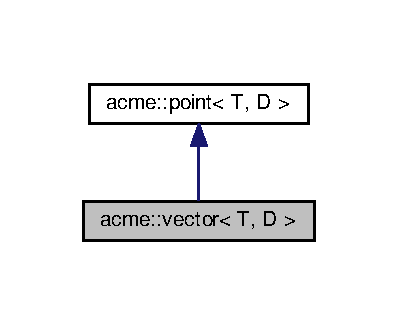
\includegraphics[width=191pt]{df/d2e/classacme_1_1vector__inherit__graph}
\end{center}
\end{figure}


Collaboration diagram for acme\+:\+:vector$<$ T, D $>$\+:\nopagebreak
\begin{figure}[H]
\begin{center}
\leavevmode
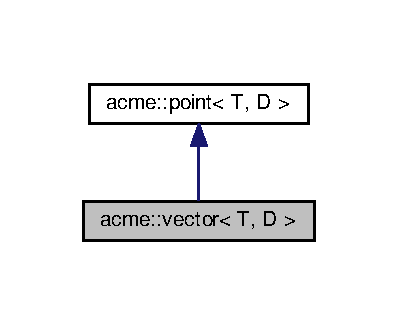
\includegraphics[width=191pt]{da/d21/classacme_1_1vector__coll__graph}
\end{center}
\end{figure}
\subsection*{Public Member Functions}
\begin{DoxyCompactItemize}
\item 
\mbox{\Hypertarget{classacme_1_1vector_af09f833651a9ddf597327a6a75a306df}\label{classacme_1_1vector_af09f833651a9ddf597327a6a75a306df}} 
\hyperlink{classacme_1_1vector_af09f833651a9ddf597327a6a75a306df}{vector} (const \hyperlink{classacme_1_1vector}{vector}$<$ T, D $>$ \&)=default
\begin{DoxyCompactList}\small\item\em Copy constructor. \end{DoxyCompactList}\item 
\mbox{\Hypertarget{classacme_1_1vector_a19de30dca513ad892825f0e49b9eb0c9}\label{classacme_1_1vector_a19de30dca513ad892825f0e49b9eb0c9}} 
\hyperlink{classacme_1_1vector_a19de30dca513ad892825f0e49b9eb0c9}{vector} ()
\begin{DoxyCompactList}\small\item\em Class constructor. \end{DoxyCompactList}\item 
\hyperlink{classacme_1_1vector_aa29b7e609acdb3ed9485a3c8864f2b5c}{vector} (const T \&v0)
\begin{DoxyCompactList}\small\item\em Class constructor for 1D vector. \end{DoxyCompactList}\item 
\hyperlink{classacme_1_1vector_a8ff8e02ac02848f92e7c8d04e6e24e85}{vector} (const T \&v0, const T \&v1)
\begin{DoxyCompactList}\small\item\em Class constructor for 2D vector. \end{DoxyCompactList}\item 
\hyperlink{classacme_1_1vector_ae5a62d7c7bb2c843014935db07c65e63}{vector} (const T \&v0, const T \&v1, const T \&v2)
\begin{DoxyCompactList}\small\item\em Class constructor for 3D vector. \end{DoxyCompactList}\item 
\hyperlink{classacme_1_1vector_a8027e03714eaada465122081b75e8d86}{vector} (const T \&v0, const T \&v1, const T \&v2, const T \&v3)
\begin{DoxyCompactList}\small\item\em Class constructor for 4D vector. \end{DoxyCompactList}\item 
\hyperlink{classacme_1_1vector_a9905548953583e0a1ef3929c4e609f8e}{vector} (const \hyperlink{classacme_1_1point}{point}$<$ T, D $>$ \&\hyperlink{classacme_1_1point}{point})
\begin{DoxyCompactList}\small\item\em Class constructor. \end{DoxyCompactList}\item 
\hyperlink{classacme_1_1vector}{vector}$<$ T, D $>$ \& \hyperlink{classacme_1_1vector_a9bf3091c36ef771c02a22e5aae144952}{operator=} (const \hyperlink{classacme_1_1vector}{vector}$<$ T, D $>$ \&\hyperlink{classacme_1_1vector}{vector})
\begin{DoxyCompactList}\small\item\em Equality operator. \end{DoxyCompactList}\item 
\mbox{\Hypertarget{classacme_1_1vector_ae8e43db3ab2dea42390d713254bb0684}\label{classacme_1_1vector_ae8e43db3ab2dea42390d713254bb0684}} 
void \hyperlink{classacme_1_1vector_ae8e43db3ab2dea42390d713254bb0684}{normalize} ()
\begin{DoxyCompactList}\small\item\em Normalize vector. \end{DoxyCompactList}\item 
\mbox{\Hypertarget{classacme_1_1vector_a067e26aadf2e8ea910a1e7b3365892cd}\label{classacme_1_1vector_a067e26aadf2e8ea910a1e7b3365892cd}} 
const \hyperlink{classacme_1_1vector}{vector}$<$ T, D $>$ \hyperlink{classacme_1_1vector_a067e26aadf2e8ea910a1e7b3365892cd}{normalized} () const
\begin{DoxyCompactList}\small\item\em Return normalized vector. \end{DoxyCompactList}\item 
\mbox{\Hypertarget{classacme_1_1point_a72a37be7ec9417b12eeec1a31ed0398b}\label{classacme_1_1point_a72a37be7ec9417b12eeec1a31ed0398b}} 
void \hyperlink{classacme_1_1point_a72a37be7ec9417b12eeec1a31ed0398b}{clear} ()
\begin{DoxyCompactList}\small\item\em Clear vector data. \end{DoxyCompactList}\item 
T \& \hyperlink{classacme_1_1point_ac8fee17f41cb01f10ecb082921018155}{operator\mbox{[}$\,$\mbox{]}} (const std\+::size\+\_\+t \&index)
\begin{DoxyCompactList}\small\item\em Indexing operator. \end{DoxyCompactList}\item 
const T \& \hyperlink{classacme_1_1point_a5e3a5ca9538fcdb337127d27fcecc2b6}{operator\mbox{[}$\,$\mbox{]}} (const std\+::size\+\_\+t \&index) const
\begin{DoxyCompactList}\small\item\em Indexing operator. \end{DoxyCompactList}\end{DoxyCompactItemize}
\subsection*{Protected Attributes}
\begin{DoxyCompactItemize}
\item 
\mbox{\Hypertarget{classacme_1_1point_a7532a61c7031fddbef1ea217cd916c4c}\label{classacme_1_1point_a7532a61c7031fddbef1ea217cd916c4c}} 
Eigen\+::\+Matrix$<$ T, D, 1 $>$ \hyperlink{classacme_1_1point_a7532a61c7031fddbef1ea217cd916c4c}{data}
\begin{DoxyCompactList}\small\item\em Point data as Eigen column vector. \end{DoxyCompactList}\end{DoxyCompactItemize}


\subsection{Detailed Description}
\subsubsection*{template$<$typename T = Float, std\+::size\+\_\+t D = 3$>$\newline
class acme\+::vector$<$ T, D $>$}

ND vector class container. 

\subsection{Constructor \& Destructor Documentation}
\mbox{\Hypertarget{classacme_1_1vector_aa29b7e609acdb3ed9485a3c8864f2b5c}\label{classacme_1_1vector_aa29b7e609acdb3ed9485a3c8864f2b5c}} 
\index{acme\+::vector@{acme\+::vector}!vector@{vector}}
\index{vector@{vector}!acme\+::vector@{acme\+::vector}}
\subsubsection{\texorpdfstring{vector()}{vector()}\hspace{0.1cm}{\footnotesize\ttfamily [1/5]}}
{\footnotesize\ttfamily template$<$typename T = Float, std\+::size\+\_\+t D = 3$>$ \\
\hyperlink{classacme_1_1vector}{acme\+::vector}$<$ T, D $>$\+::\hyperlink{classacme_1_1vector}{vector} (\begin{DoxyParamCaption}\item[{const T \&}]{v0 }\end{DoxyParamCaption})\hspace{0.3cm}{\ttfamily [inline]}}



Class constructor for 1D vector. 


\begin{DoxyParams}{Parameters}
{\em v0} & Input value 0 \\
\hline
\end{DoxyParams}
\mbox{\Hypertarget{classacme_1_1vector_a8ff8e02ac02848f92e7c8d04e6e24e85}\label{classacme_1_1vector_a8ff8e02ac02848f92e7c8d04e6e24e85}} 
\index{acme\+::vector@{acme\+::vector}!vector@{vector}}
\index{vector@{vector}!acme\+::vector@{acme\+::vector}}
\subsubsection{\texorpdfstring{vector()}{vector()}\hspace{0.1cm}{\footnotesize\ttfamily [2/5]}}
{\footnotesize\ttfamily template$<$typename T = Float, std\+::size\+\_\+t D = 3$>$ \\
\hyperlink{classacme_1_1vector}{acme\+::vector}$<$ T, D $>$\+::\hyperlink{classacme_1_1vector}{vector} (\begin{DoxyParamCaption}\item[{const T \&}]{v0,  }\item[{const T \&}]{v1 }\end{DoxyParamCaption})\hspace{0.3cm}{\ttfamily [inline]}}



Class constructor for 2D vector. 


\begin{DoxyParams}{Parameters}
{\em v0} & Input value 0 \\
\hline
{\em v1} & Input value 1 \\
\hline
\end{DoxyParams}
\mbox{\Hypertarget{classacme_1_1vector_ae5a62d7c7bb2c843014935db07c65e63}\label{classacme_1_1vector_ae5a62d7c7bb2c843014935db07c65e63}} 
\index{acme\+::vector@{acme\+::vector}!vector@{vector}}
\index{vector@{vector}!acme\+::vector@{acme\+::vector}}
\subsubsection{\texorpdfstring{vector()}{vector()}\hspace{0.1cm}{\footnotesize\ttfamily [3/5]}}
{\footnotesize\ttfamily template$<$typename T = Float, std\+::size\+\_\+t D = 3$>$ \\
\hyperlink{classacme_1_1vector}{acme\+::vector}$<$ T, D $>$\+::\hyperlink{classacme_1_1vector}{vector} (\begin{DoxyParamCaption}\item[{const T \&}]{v0,  }\item[{const T \&}]{v1,  }\item[{const T \&}]{v2 }\end{DoxyParamCaption})\hspace{0.3cm}{\ttfamily [inline]}}



Class constructor for 3D vector. 


\begin{DoxyParams}{Parameters}
{\em v0} & Input value 0 \\
\hline
{\em v1} & Input value 1 \\
\hline
{\em v2} & Input value 2 \\
\hline
\end{DoxyParams}
\mbox{\Hypertarget{classacme_1_1vector_a8027e03714eaada465122081b75e8d86}\label{classacme_1_1vector_a8027e03714eaada465122081b75e8d86}} 
\index{acme\+::vector@{acme\+::vector}!vector@{vector}}
\index{vector@{vector}!acme\+::vector@{acme\+::vector}}
\subsubsection{\texorpdfstring{vector()}{vector()}\hspace{0.1cm}{\footnotesize\ttfamily [4/5]}}
{\footnotesize\ttfamily template$<$typename T = Float, std\+::size\+\_\+t D = 3$>$ \\
\hyperlink{classacme_1_1vector}{acme\+::vector}$<$ T, D $>$\+::\hyperlink{classacme_1_1vector}{vector} (\begin{DoxyParamCaption}\item[{const T \&}]{v0,  }\item[{const T \&}]{v1,  }\item[{const T \&}]{v2,  }\item[{const T \&}]{v3 }\end{DoxyParamCaption})\hspace{0.3cm}{\ttfamily [inline]}}



Class constructor for 4D vector. 


\begin{DoxyParams}{Parameters}
{\em v0} & Input value 0 \\
\hline
{\em v1} & Input value 1 \\
\hline
{\em v2} & Input value 2 \\
\hline
{\em v3} & Input value 3 \\
\hline
\end{DoxyParams}
\mbox{\Hypertarget{classacme_1_1vector_a9905548953583e0a1ef3929c4e609f8e}\label{classacme_1_1vector_a9905548953583e0a1ef3929c4e609f8e}} 
\index{acme\+::vector@{acme\+::vector}!vector@{vector}}
\index{vector@{vector}!acme\+::vector@{acme\+::vector}}
\subsubsection{\texorpdfstring{vector()}{vector()}\hspace{0.1cm}{\footnotesize\ttfamily [5/5]}}
{\footnotesize\ttfamily template$<$typename T = Float, std\+::size\+\_\+t D = 3$>$ \\
\hyperlink{classacme_1_1vector}{acme\+::vector}$<$ T, D $>$\+::\hyperlink{classacme_1_1vector}{vector} (\begin{DoxyParamCaption}\item[{const \hyperlink{classacme_1_1point}{point}$<$ T, D $>$ \&}]{point }\end{DoxyParamCaption})\hspace{0.3cm}{\ttfamily [inline]}}



Class constructor. 


\begin{DoxyParams}{Parameters}
{\em point} & Input ND point \\
\hline
\end{DoxyParams}


\subsection{Member Function Documentation}
\mbox{\Hypertarget{classacme_1_1vector_a9bf3091c36ef771c02a22e5aae144952}\label{classacme_1_1vector_a9bf3091c36ef771c02a22e5aae144952}} 
\index{acme\+::vector@{acme\+::vector}!operator=@{operator=}}
\index{operator=@{operator=}!acme\+::vector@{acme\+::vector}}
\subsubsection{\texorpdfstring{operator=()}{operator=()}}
{\footnotesize\ttfamily template$<$typename T = Float, std\+::size\+\_\+t D = 3$>$ \\
\hyperlink{classacme_1_1vector}{vector}$<$T, D$>$\& \hyperlink{classacme_1_1vector}{acme\+::vector}$<$ T, D $>$\+::operator= (\begin{DoxyParamCaption}\item[{const \hyperlink{classacme_1_1vector}{vector}$<$ T, D $>$ \&}]{vector }\end{DoxyParamCaption})\hspace{0.3cm}{\ttfamily [inline]}}



Equality operator. 


\begin{DoxyParams}{Parameters}
{\em vector} & Input ND point \\
\hline
\end{DoxyParams}
\mbox{\Hypertarget{classacme_1_1point_ac8fee17f41cb01f10ecb082921018155}\label{classacme_1_1point_ac8fee17f41cb01f10ecb082921018155}} 
\index{acme\+::vector@{acme\+::vector}!operator\mbox{[}\mbox{]}@{operator[]}}
\index{operator\mbox{[}\mbox{]}@{operator[]}!acme\+::vector@{acme\+::vector}}
\subsubsection{\texorpdfstring{operator[]()}{operator[]()}\hspace{0.1cm}{\footnotesize\ttfamily [1/2]}}
{\footnotesize\ttfamily template$<$typename T = Float, std\+::size\+\_\+t D = 3$>$ \\
T\& \hyperlink{classacme_1_1point}{acme\+::point}$<$ T, D $>$\+::operator\mbox{[}$\,$\mbox{]} (\begin{DoxyParamCaption}\item[{const std\+::size\+\_\+t \&}]{index }\end{DoxyParamCaption})\hspace{0.3cm}{\ttfamily [inline]}, {\ttfamily [inherited]}}



Indexing operator. 


\begin{DoxyParams}{Parameters}
{\em index} & Input index \\
\hline
\end{DoxyParams}
\mbox{\Hypertarget{classacme_1_1point_a5e3a5ca9538fcdb337127d27fcecc2b6}\label{classacme_1_1point_a5e3a5ca9538fcdb337127d27fcecc2b6}} 
\index{acme\+::vector@{acme\+::vector}!operator\mbox{[}\mbox{]}@{operator[]}}
\index{operator\mbox{[}\mbox{]}@{operator[]}!acme\+::vector@{acme\+::vector}}
\subsubsection{\texorpdfstring{operator[]()}{operator[]()}\hspace{0.1cm}{\footnotesize\ttfamily [2/2]}}
{\footnotesize\ttfamily template$<$typename T = Float, std\+::size\+\_\+t D = 3$>$ \\
const T\& \hyperlink{classacme_1_1point}{acme\+::point}$<$ T, D $>$\+::operator\mbox{[}$\,$\mbox{]} (\begin{DoxyParamCaption}\item[{const std\+::size\+\_\+t \&}]{index }\end{DoxyParamCaption}) const\hspace{0.3cm}{\ttfamily [inline]}, {\ttfamily [inherited]}}



Indexing operator. 


\begin{DoxyParams}{Parameters}
{\em index} & Input index \\
\hline
\end{DoxyParams}


The documentation for this class was generated from the following file\+:\begin{DoxyCompactItemize}
\item 
src/acme\+\_\+vector.\+hh\end{DoxyCompactItemize}

%--- End generated contents ---

% Index
\backmatter
\newpage
\phantomsection
\clearemptydoublepage
\addcontentsline{toc}{chapter}{Index}
\printindex

\end{document}
